% !TeX program = xelatex
\documentclass[9pt]{beamer}
\usepackage{xcolor}
\definecolor{orange}{HTML}{F67941}
\definecolor{red}{HTML}{AC454A}
\definecolor{brown}{HTML}{EAD296}
\definecolor{darkgrey}{HTML}{313630}
\usefonttheme{professionalfonts} % using non standard fonts for beamer
\usefonttheme{serif} % default family is serif
\usepackage{fontspec}
\usepackage{setspace}
\usepackage{natbib}
%\usepackage[T1]{fontenc}

\bibliographystyle{abbrv}
%\setmainfont{Liberation Serif}
%\setmainfont{Liberation Serif}
\setmainfont{Comfortaa}
%\usepackage[T1]{fontenc}

\setbeamercolor{frametitle}{bg=orange,fg=white}
\setbeamercolor{author in head/foot}{bg=orange,fg=white}

%\setbeamerfont{page number}{size=\Huge}

%\setbeamertemplate{itemize items}[circle]
\useinnertheme{circles}
\setbeamercolor{palette primary}{bg=orange,fg=white}
%\setbeamercolor{palette secondary}{bg=red,fg=white}
\setbeamertemplate{itemize item}{\color{darkgrey}$\circ$}
\setbeamercolor{structure}{fg=red} % itemize, enumerate, etc

%\setbeamercolor{section in head/foot}{bg=red}
\setbeamercolor{title}{fg=orange} %, bg=brown
\setbeamercolor{author}{fg=darkgrey}
\setbeamercolor{institute}{fg=darkgrey}
\setbeamercolor{date}{fg=darkgrey}
%\setbeamercolor{normal text}{fg=darkgrey}
\makeatletter
\setbeamertemplate{headline}{%
	\usebeamercolor[bg]{frametitle}\rule{\textwidth}{1cm}
}
\setbeamerfont{title}{size=\LARGE}
\setbeamerfont{institute}{size=\normalsize}
\renewcommand*{\bibfont}{\scriptsize}


\setbeamertemplate{frametitle}{%
	\vskip-1cm%
	\begin{minipage}[c][\headheight][c]{\textwidth}%
		\usebeamerfont{frametitle}
		\strut\insertframetitle\par
		{%
			\ifx\insertframesubtitle\@empty%
			\else%
			{\usebeamerfont{framesubtitle}\usebeamercolor[fg]{framesubtitle}\strut\insertframesubtitle\par}%
			\fi
		}%      
		\vspace*{0.05cm}
	\end{minipage}%
	\vskip-0.1em
}
%\setbeamertemplate{footline}{%
%	\leavevmode%
%	\hbox{\begin{beamercolorbox}[wd=\paperwidth,ht=4.5ex,dp=3.125ex]{author in head/foot}%
%			\usebeamerfont{author in head/foot} bar
%	\end{beamercolorbox}}%
%	\vskip0pt%
%}
\makeatother


\title{Uncertainty in\\Recurrent Decision Tree Classifiers}
\author{Stefan Wezel}
\institute{Explainable Machine Learning}
\date{\today}


%\setbeamertemplate{sidebar right}{}
%\setbeamertemplate{footline}{%
%	\hfill\usebeamertemplate***{navigation symbols}
%	\hspace{1cm}\insertframenumber{}}
\setbeamerfont{page number in head/foot}{size=\small}
    \setbeamertemplate{footline}{%
	\raisebox{5pt}{\makebox[\paperwidth]{\hfill\makebox[10pt]{\scriptsize\insertframenumber}}}}
\setbeamertemplate{navigation symbols}{}
%\onehalfspacing
\setstretch{1.3}
\begin{document}
	

\setbeamercolor{background canvas}{bg=white}
\setbeamercolor{normal text}{fg=darkgrey}
\usebeamercolor[fg]{normal text}
\begin{frame}[plain]
	\titlepage
\end{frame} 

\setbeamercolor{background canvas}{bg=white}
\setbeamercolor{normal text}{fg=darkgrey}
\usebeamercolor[fg]{normal text}
\setbeamertemplate{itemize item}{\color{darkgrey}$\circ$}
\begin{frame}
\frametitle{What?}
\framesubtitle{Setting}
	\begin{itemize}%\setlength\itemsep{1.5em}
	\item Many powerful architectures for image classification
	\item Prominent example: ResNet
	\item Popular models only yield classification
	\item No reasoning behind classification
	\end{itemize}
\end{frame} 


\setbeamercolor{background canvas}{bg=white}
\setbeamercolor{normal text}{fg=darkgrey}
\usebeamercolor[fg]{normal text}
\setbeamertemplate{itemize item}{\color{darkgrey}$\circ$}
\begin{frame}
\frametitle{What?}
\framesubtitle{What is a Recurrent Decision Tree Classifier?}
	\begin{figure}
	\centering
	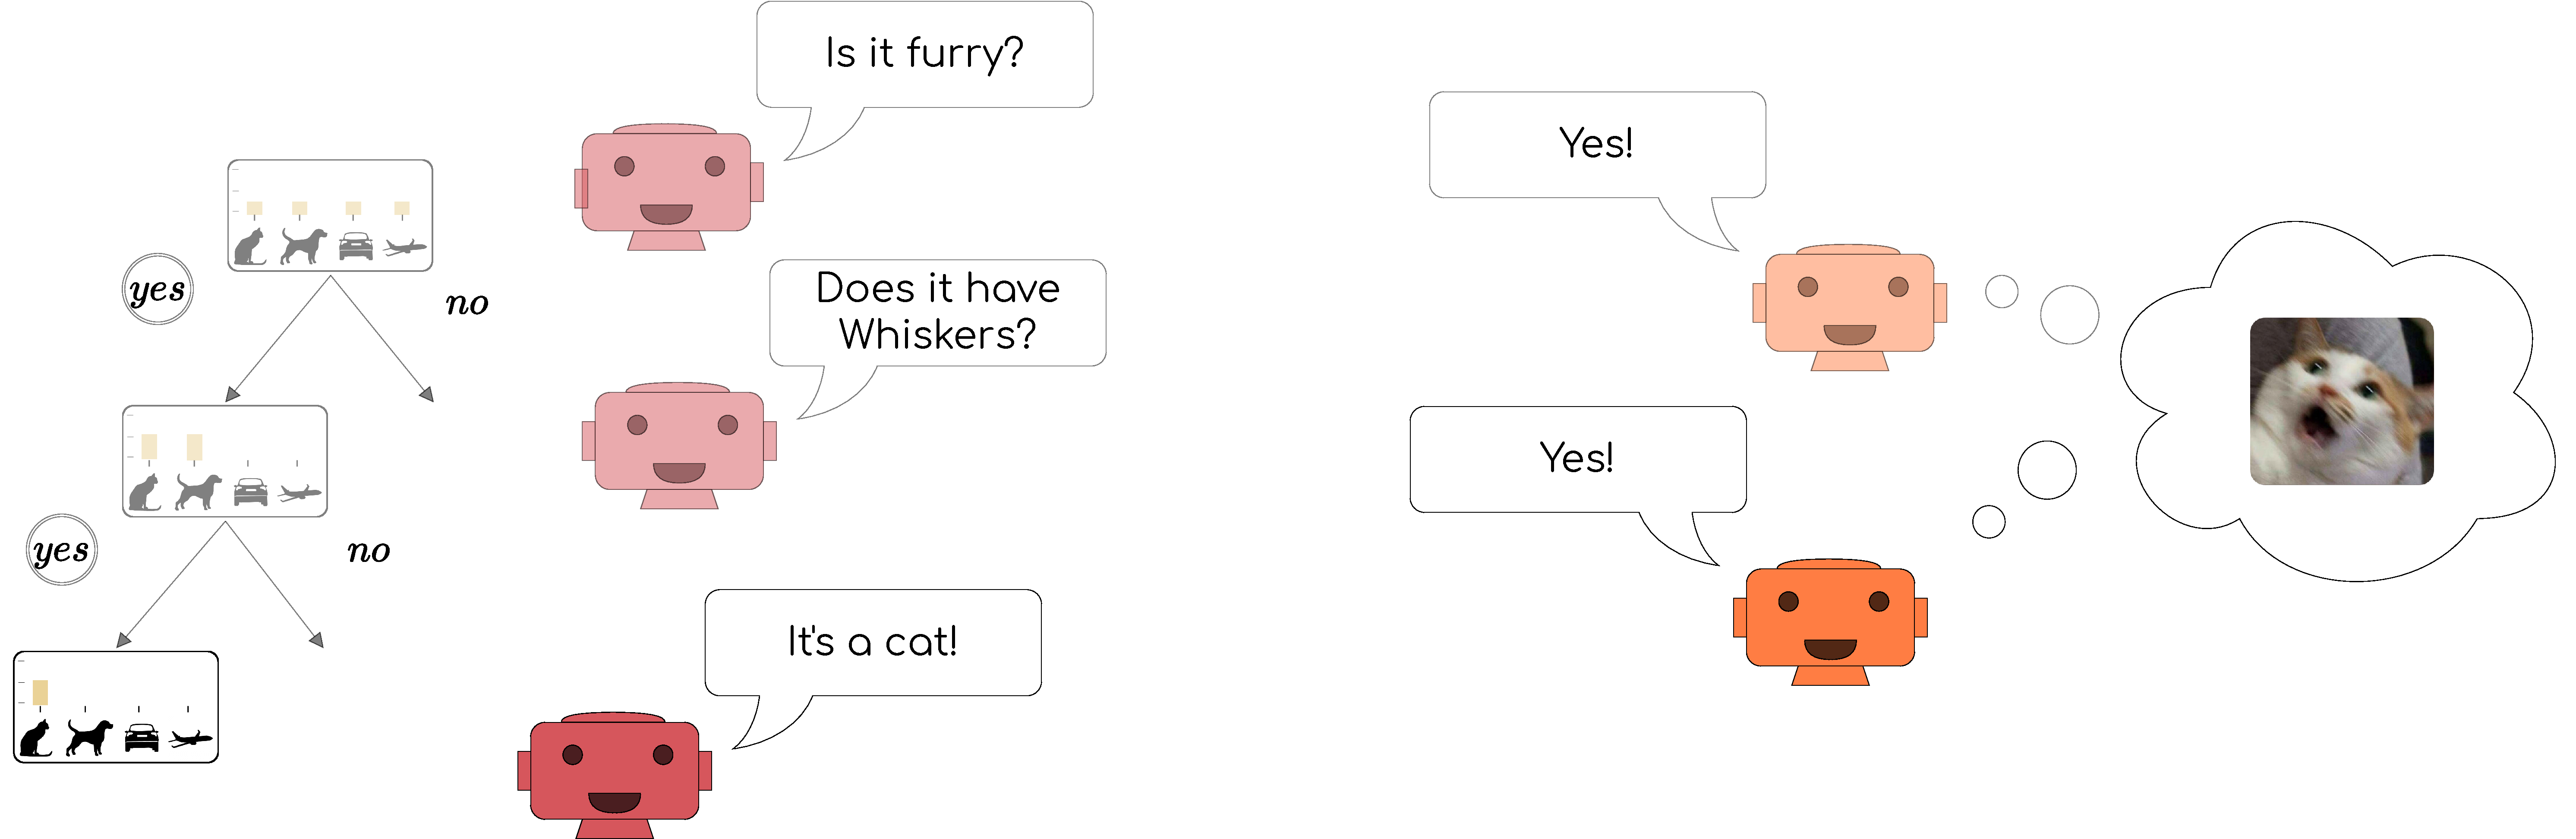
\includegraphics[width=1\textwidth]{images/rdtc_intuition.pdf}
	%\caption[caption for ]{After collecting images of birds, the ornithologist lets our proposed model classify the vast amount of data. Only in cases of high uncertainty, she is consulted and can classify the image manually. \footnotemark}
	%\label{fig:qual}
\end{figure}
\begin{itemize}%\setlength\itemsep{1em}
	\item Alaniz and Akata \cite{alaniz2019explainable} propose RDTC
	\item Two communicating agents
	\item Left: ask questions ---- right: look at data and answer them
	\item Unfolding tree reveals reasoning behind classification
\end{itemize}
\end{frame} 


\setbeamercolor{background canvas}{bg=white}
\setbeamercolor{normal text}{fg=darkgrey}
\usebeamercolor[fg]{normal text}
\setbeamertemplate{itemize item}{\color{darkgrey}$\circ$}	
\begin{frame}
\frametitle{What?}
\framesubtitle{Introducing Uncertainty to a RDTC}
\begin{figure}
	\centering
	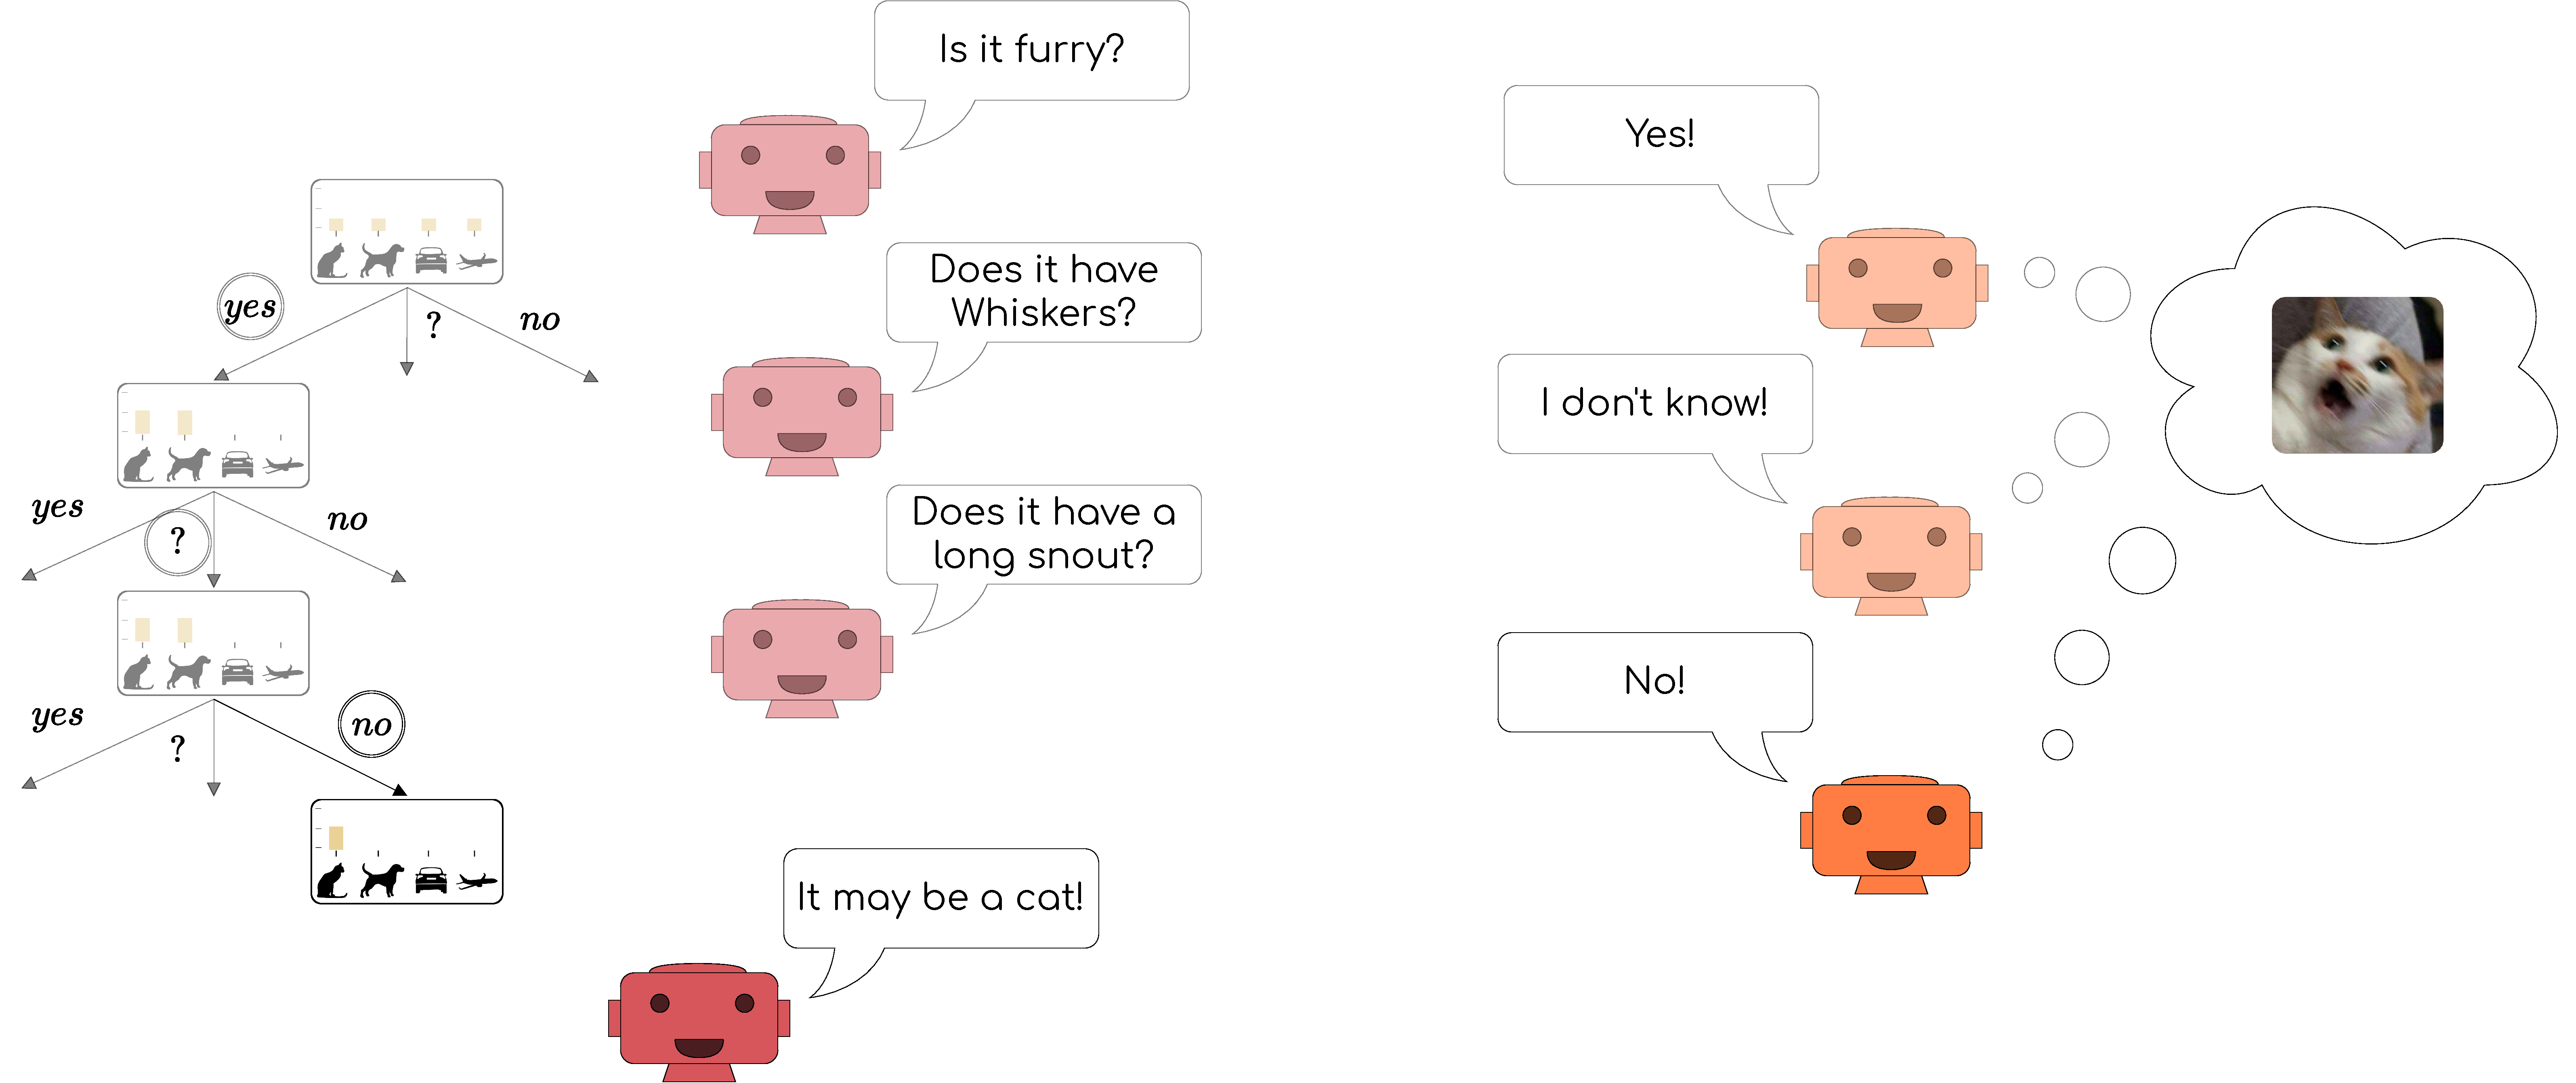
\includegraphics[width=1\textwidth]{images/urdtc_intuition.pdf}
	%\caption[caption for ]{After collecting images of birds, the ornithologist lets our proposed model classify the vast amount of data. Only in cases of high uncertainty, she is consulted and can classify the image manually. \footnotemark}
	%\label{fig:qual}
\end{figure}
\begin{itemize}%\setlength\itemsep{1em}
	%\item The agent, seeing the data becomes aware of its uncertainty which is communicated to the other agent
	\item Right agent is aware of uncertainties
	\item Communicates this to left agent
\end{itemize}
\end{frame} 



\setbeamercolor{background canvas}{bg=white}
\setbeamercolor{normal text}{fg=darkgrey}
\usebeamercolor[fg]{normal text}
\setbeamertemplate{itemize item}{\color{darkgrey}$\circ$}
\begin{frame}
\frametitle{Why do we need uncertainty?}
\framesubtitle{A Practical Example...}
	\begin{figure}
		\centering
		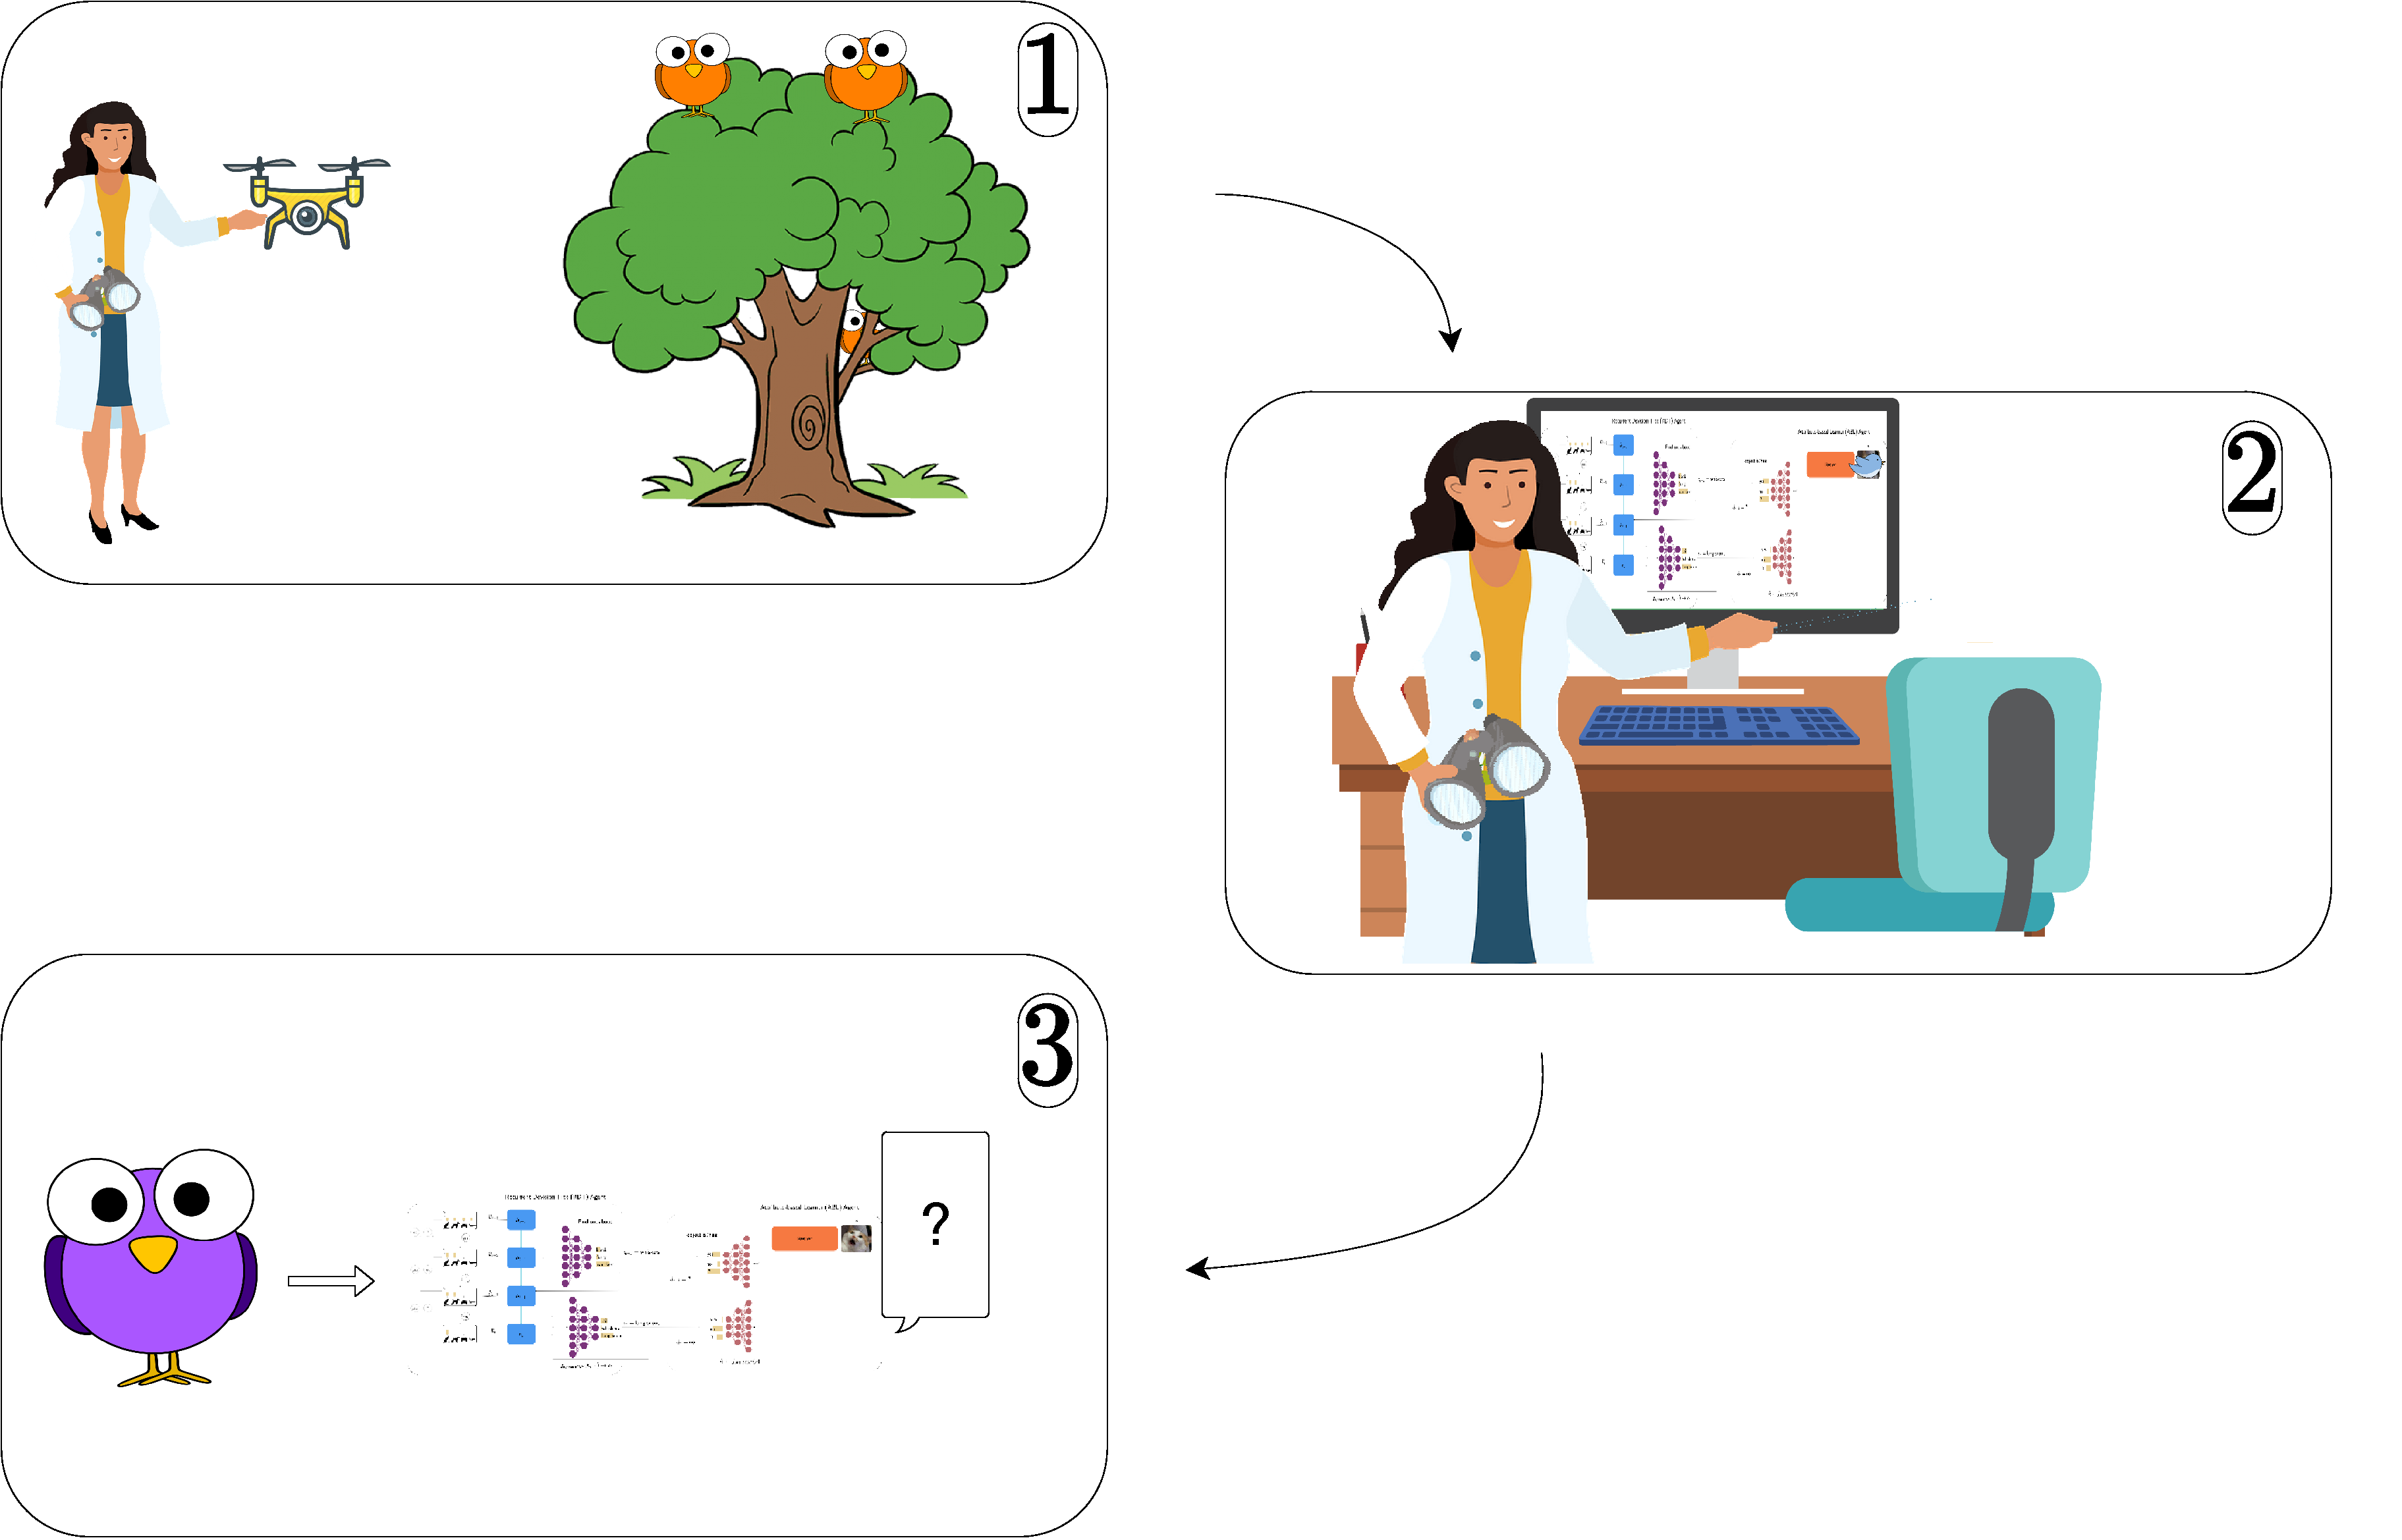
\includegraphics[width=0.6\textwidth]{images/ornithology.pdf}
		%\caption[caption for ]{After collecting images of birds, the ornithologist lets our proposed model classify the vast amount of data. Only in cases of high uncertainty, she is consulted and can classify the image manually. \footnotemark}
		%\label{fig:qual}
	\end{figure}
	\begin{itemize}%\setlength\itemsep{1em}
	\item Ornithologist surveys area using drone and CV software
	\item Classification is automated with our model
	\item Bird species unknown to model yield high uncertainty
	\item Those can be classified manually
	\end{itemize}
\end{frame}

\setbeamercolor{background canvas}{bg=orange}
\setbeamercolor{normal text}{fg=white}	
\usebeamercolor[fg]{normal text}
\setbeamertemplate{itemize item}{\color{white}$\circ$}
\begin{frame}
\frametitle{Introduction}
\begin{itemize}
	\item RDTC by Alaniz and Akata \cite{alaniz2019explainable} yields decision tree
	\item Decision tree is build through communication of agents
	\item Our aim is to introduce uncertainty to RDTC
	\item Uncertainty allows model to i.e. detect OOD examples
	%\item This is useful in settings where high-risk decision can be consequential
\end{itemize}
\end{frame}
%\setbeamertemplate{background canvas}{bg=white}



\setbeamercolor{background canvas}{bg=white}
\setbeamercolor{normal text}{fg=darkgrey}
\usebeamercolor[fg]{normal text}
\setbeamertemplate{itemize item}{\color{darkgrey}$\circ$}
\begin{frame}
\frametitle{How?}
\framesubtitle{Architecture}
\begin{figure}
	\centering
	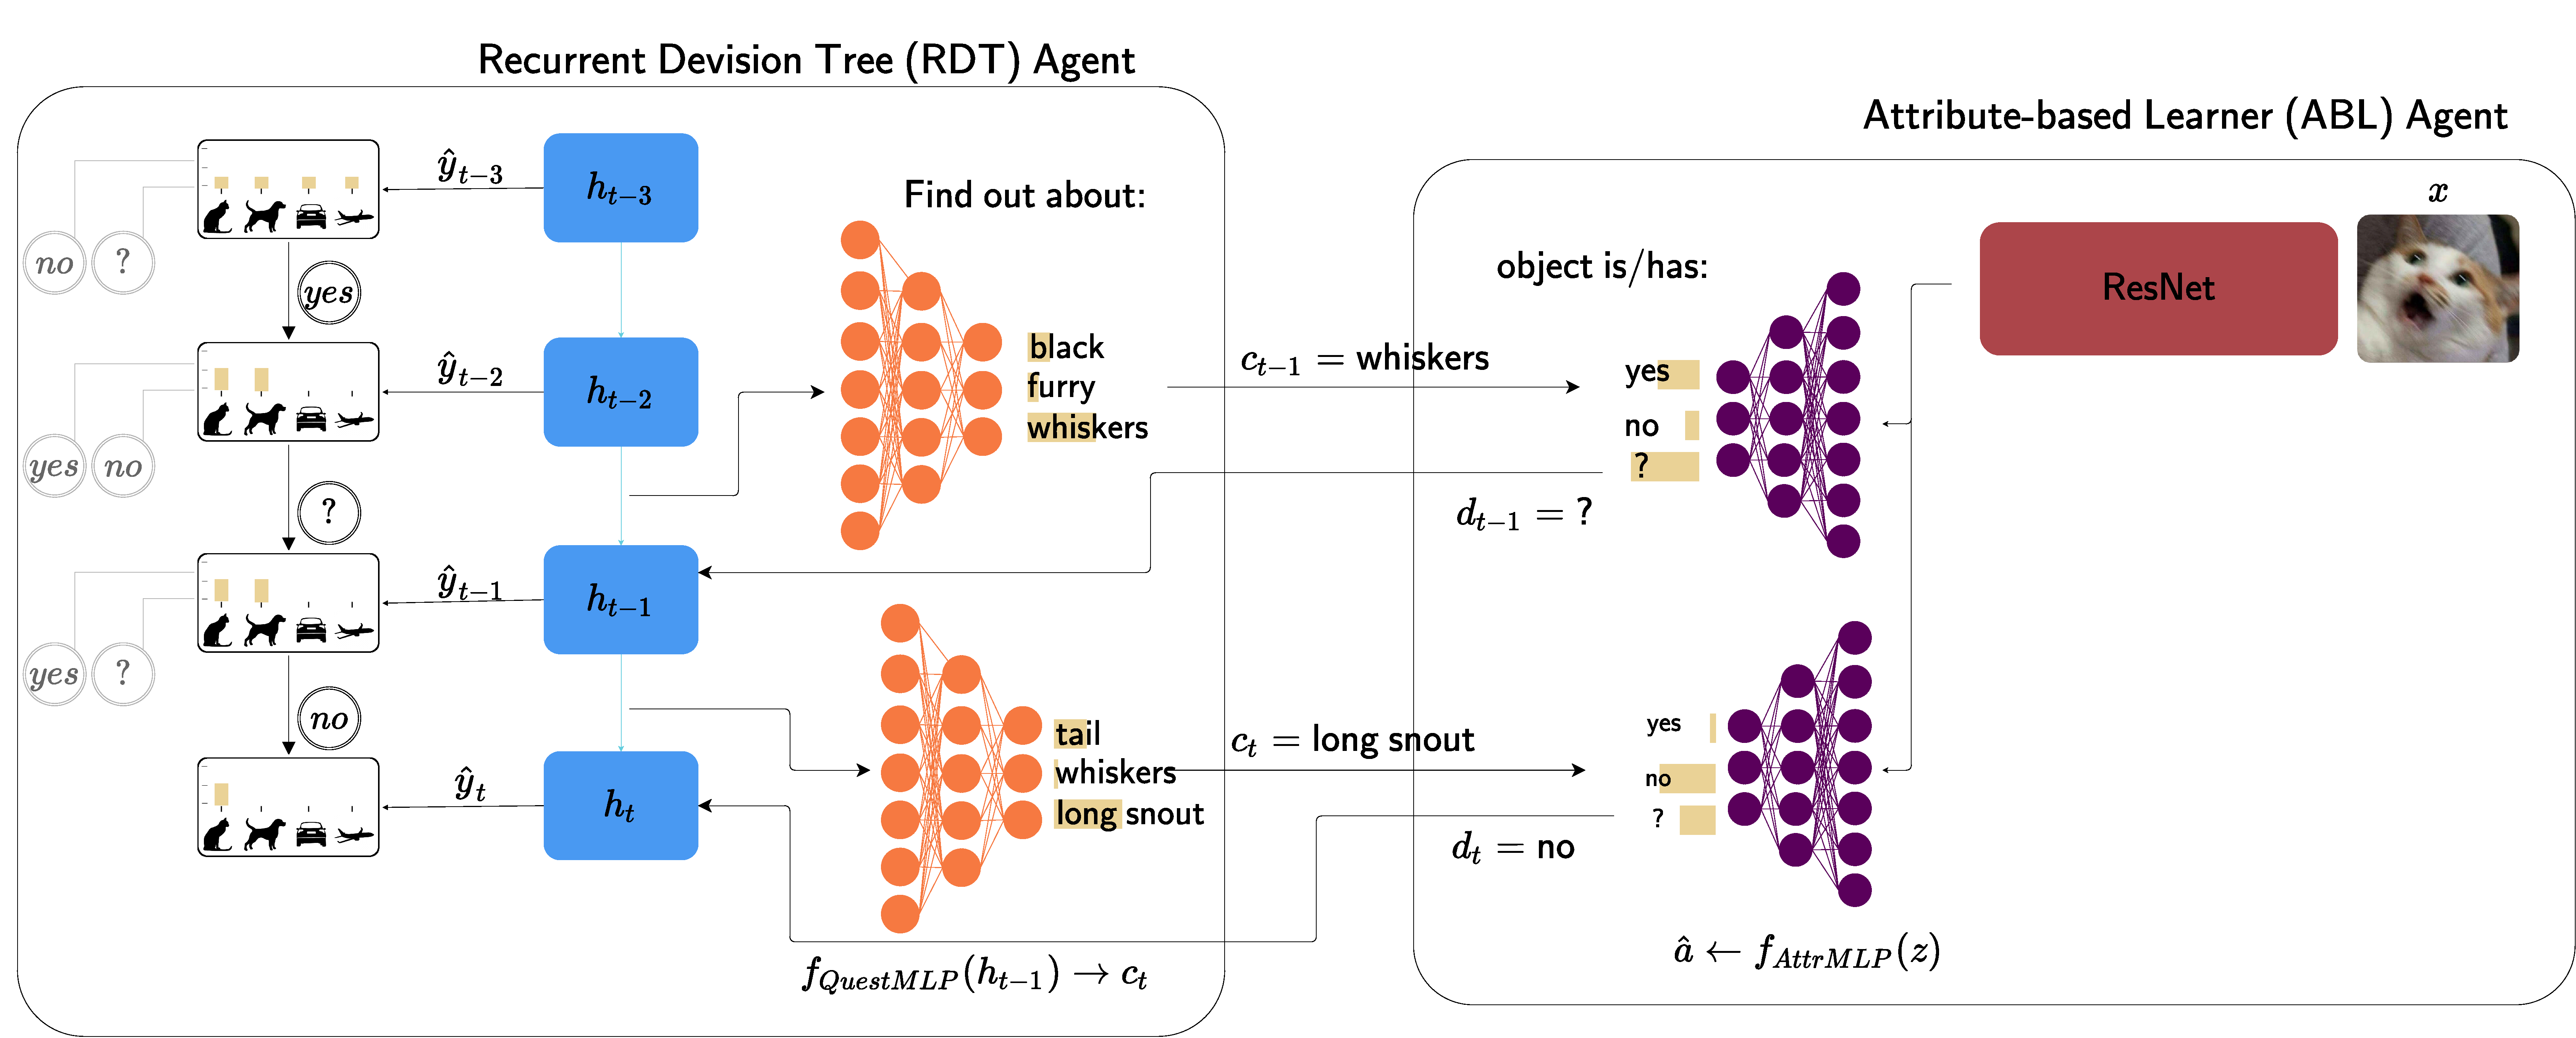
\includegraphics[width=0.9\textwidth]{images/uncertaintRDTC.pdf} 
	%\caption{The RDT asks questions about presence, absence or uncertainty of attributes. The answers, given by the AbL are used by the RDT agent to make a classification each iteration.}
	\label{fig:uncertainRDTC}
\end{figure}
\begin{itemize}
	\item RDT can not see the images and only ask if attribute is present
	\item The AbL can see the image and answer RDT's questions
\end{itemize}
\end{frame} 





%AbL
\setbeamercolor{background canvas}{bg=white}
\setbeamercolor{normal text}{fg=darkgrey}
\usebeamercolor[fg]{normal text}
\setbeamertemplate{itemize item}{\color{darkgrey}$\circ$}
\begin{frame}
\frametitle{Attribute-based Learner}
\framesubtitle{Answering questions}
\begin{itemize}
	\item Extract features from image using ResNet
	\item MLP maps features to 'yes-no' answers
	\item those indicate absence/presence of attributes
	%\item It returns a tensor with the of shape number of attributes $\times$ decision size
	\item Discrete answer from AbL though applying \begin{align*}
	&TempSoftmax(log\;\pi) = \frac{exp((log\;\pi_i)/\tau)}{\sum_{j=1}^{K}exp((log\;\pi_j)/\tau)} = d_t
	\text{ on }
	log\;\pi \\
	&\text{ which are logit values for either 'Yes', or 'No' per attribute.}
\end{align*}
\item TempSoftmax as differentiable approximation to argmax
\end{itemize}
\end{frame}


%RDT
\setbeamercolor{background canvas}{bg=white}
\setbeamercolor{normal text}{fg=darkgrey}
\usebeamercolor[fg]{normal text}
\setbeamertemplate{itemize item}{\color{darkgrey}$\circ$}	
\begin{frame}
\frametitle{Recurrent Decision Tree}
\framesubtitle{Building a decision tree}
\begin{itemize}
%	\item The RDT consists of several models:
		\item LSTM
		\begin{itemize}
			\item Hidden state based on previous hidden states and new answers
		\end{itemize}
		\item Explicit Memory
		\begin{itemize}
			\item Stores all questions and corresponding answers
			\item Its content is the decision tree
		\end{itemize}
		\item $f_{ClassMLP}$
		\begin{itemize}
			\item Make classification based on LSTM's hidden state
		\end{itemize}
		\item $f_{QuestMLP}$
		\begin{itemize}
			\item Find next question to ask based on LSTM's hidden state
			\item Next question is the index the $f_{QuestMLP}$ poses
			\item To turn logits into a discrete value, Gumbel softmax is used
			\item This allows us to sample an index from the logits
			\item \begin{align*}
				GumbelSoftmax(log\;\pi) &= \frac{exp((log\;\pi_i + g_i)/\tau)}{\sum_{j=1}^{K}exp((log\;\pi_j + g_j)/\tau)}
			\end{align*}
		\end{itemize}
		
\end{itemize}
\end{frame}
\setbeamercolor{background canvas}{bg=white}
\setbeamercolor{normal text}{fg=darkgrey}
\usebeamercolor[fg]{normal text}
\setbeamertemplate{itemize item}{\color{darkgrey}$\circ$}
\begin{frame}
\frametitle{Attribute-based Learner}
\framesubtitle{Extracting features}
\begin{columns}[T]
	\begin{column}{.5\textwidth}
		\begin{itemize}
			\item Extract features using ResNet
			\item Then pass to $f_{AttrMLP}$
			% Your text here
		\end{itemize}
	\end{column}
	\begin{column}{.5\textwidth}
		% Your image included here
		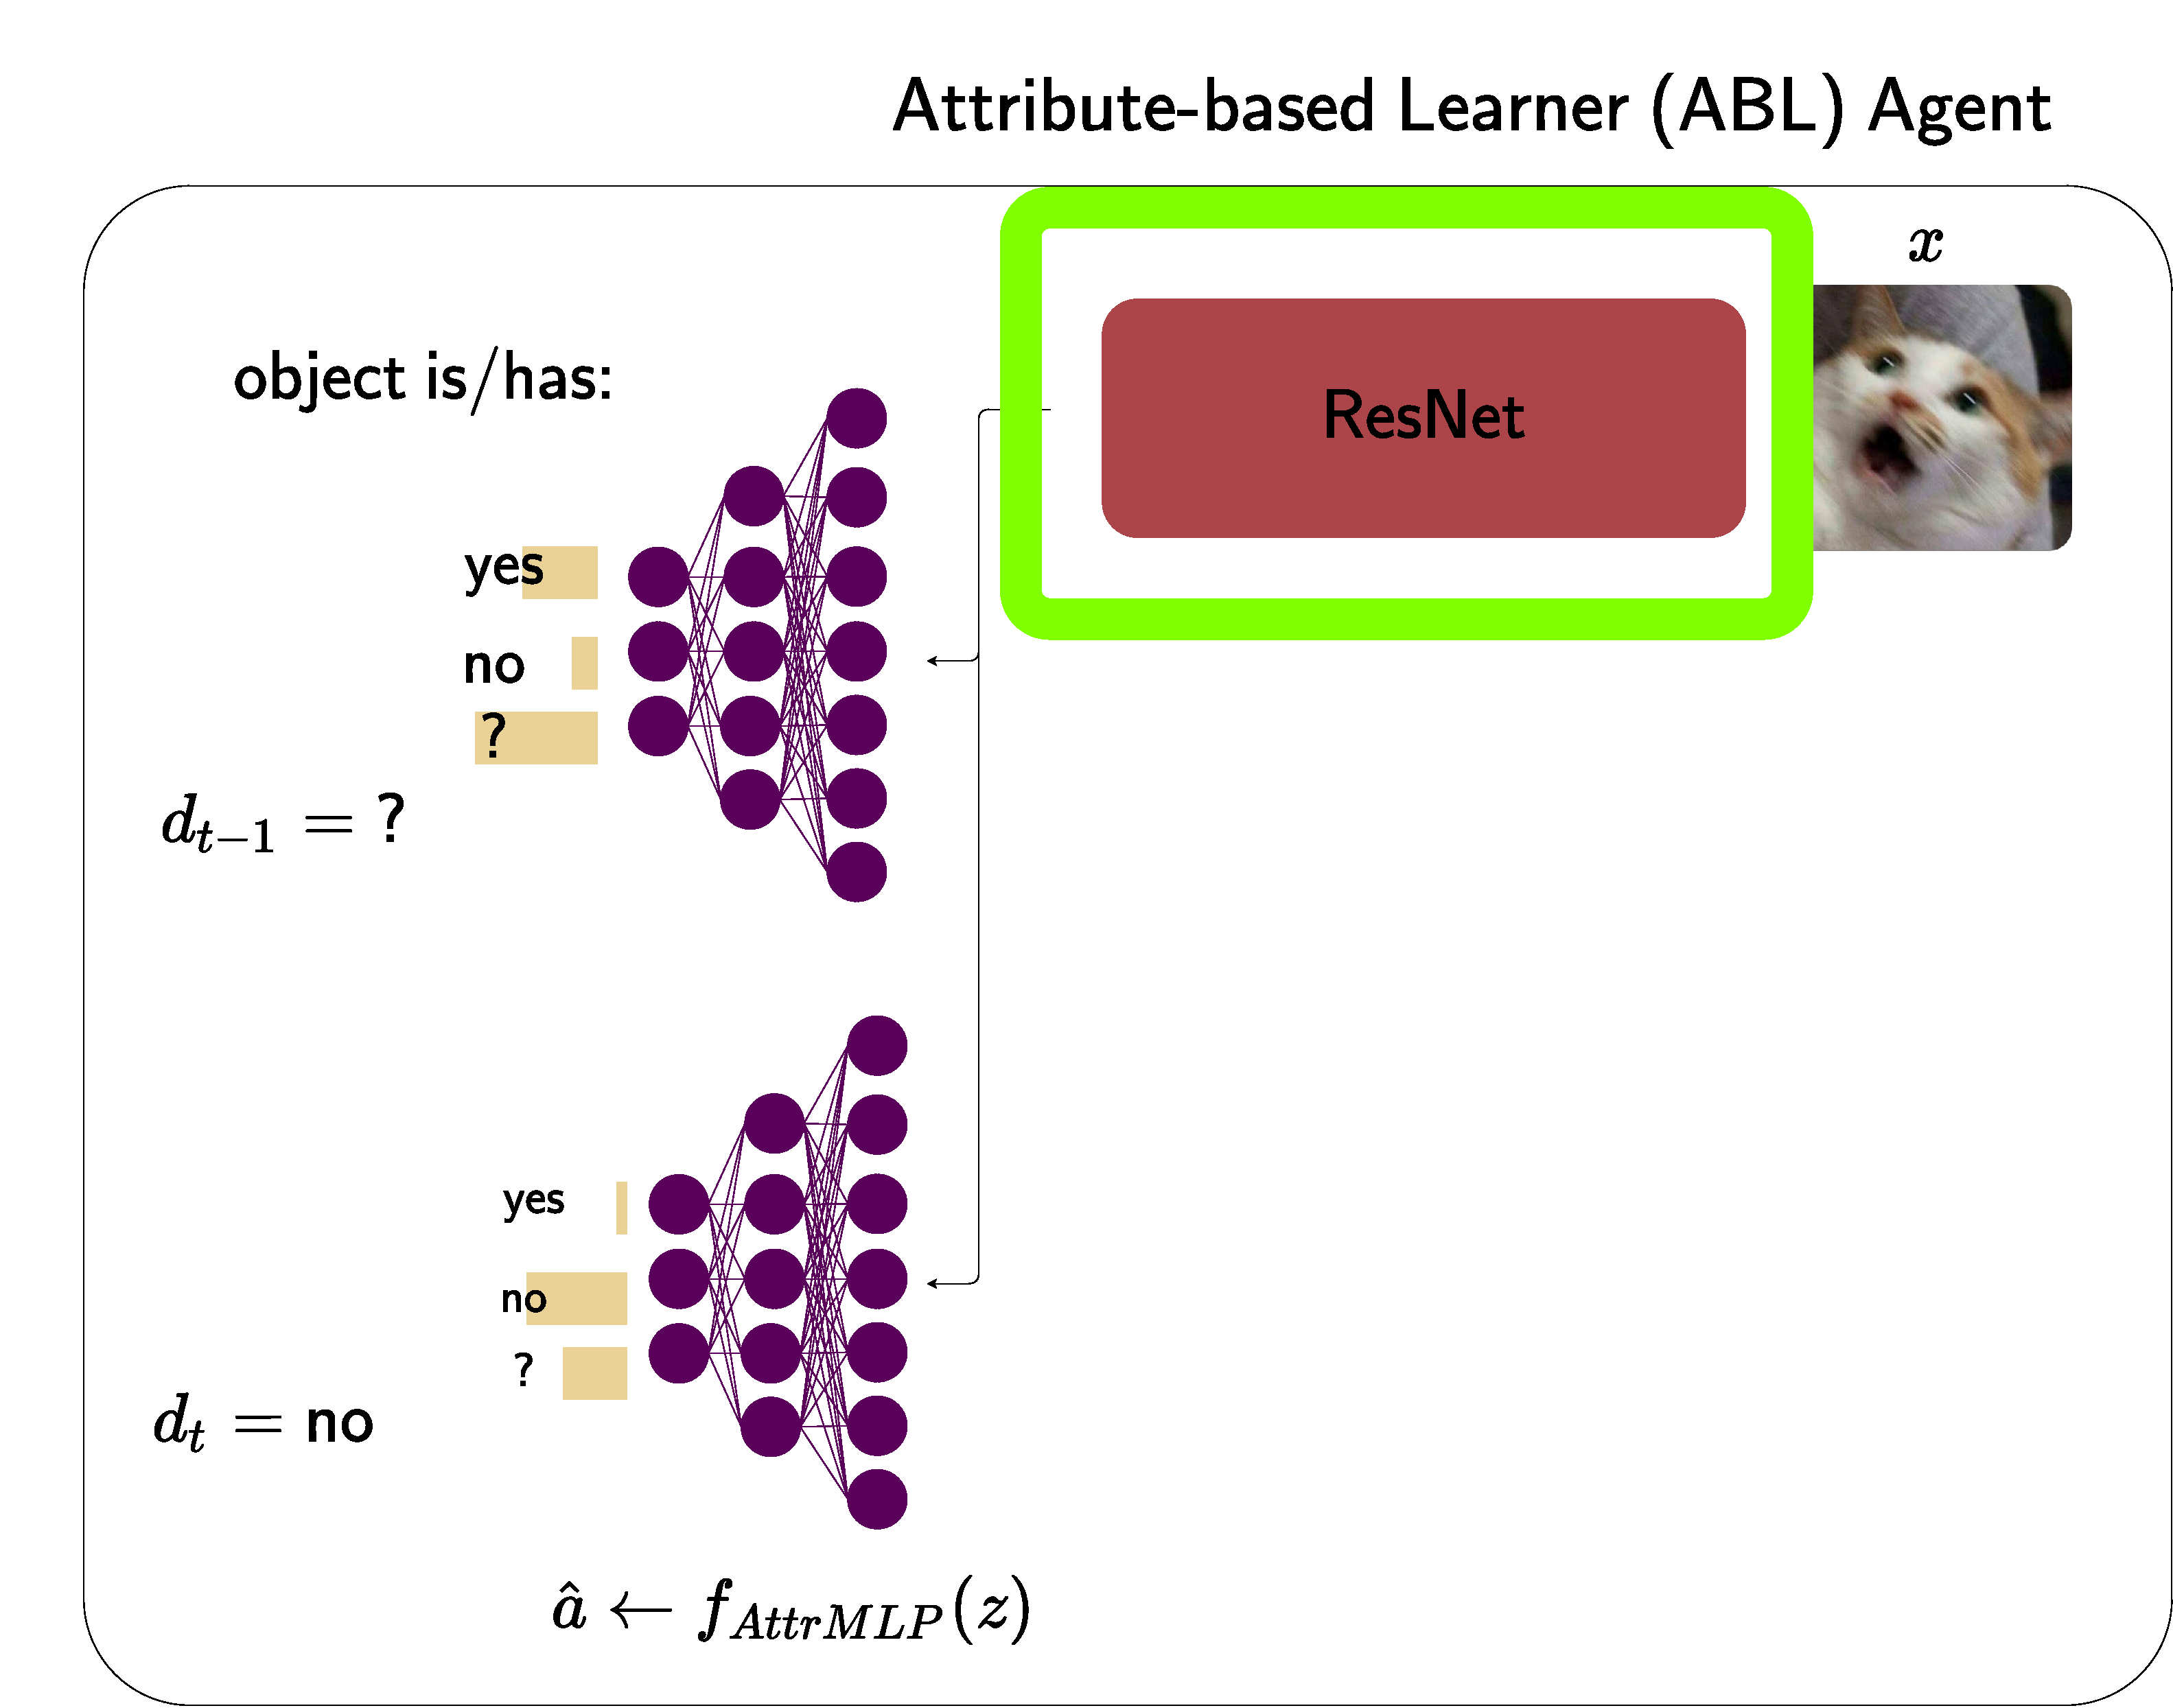
\includegraphics[width=\textwidth]{images/urdtc_parts_resnet.pdf}
	\end{column}
\end{columns}
\end{frame}

\setbeamercolor{background canvas}{bg=white}
\setbeamercolor{normal text}{fg=darkgrey}
\usebeamercolor[fg]{normal text}
\setbeamertemplate{itemize item}{\color{darkgrey}$\circ$}
\begin{frame}
\frametitle{Attribute-based Learner}
\framesubtitle{Mapping features to attributes}
\begin{columns}[T]
\begin{column}{.5\textwidth}
	\begin{itemize}
		\item Map features to answers
		\item Yes, No, ? for each attribute
		\item Discrete answers with TempSoftmax
		\begin{align*}
		&\frac{exp((log\;\pi_i)/\tau)}{\sum_{j=1}^{K}exp((log\;\pi_j)/\tau)}\\
		& = \hat{a}
		\end{align*}
		% Your text here
	\end{itemize}
\end{column}
\begin{column}{.5\textwidth}
	% Your image included here
	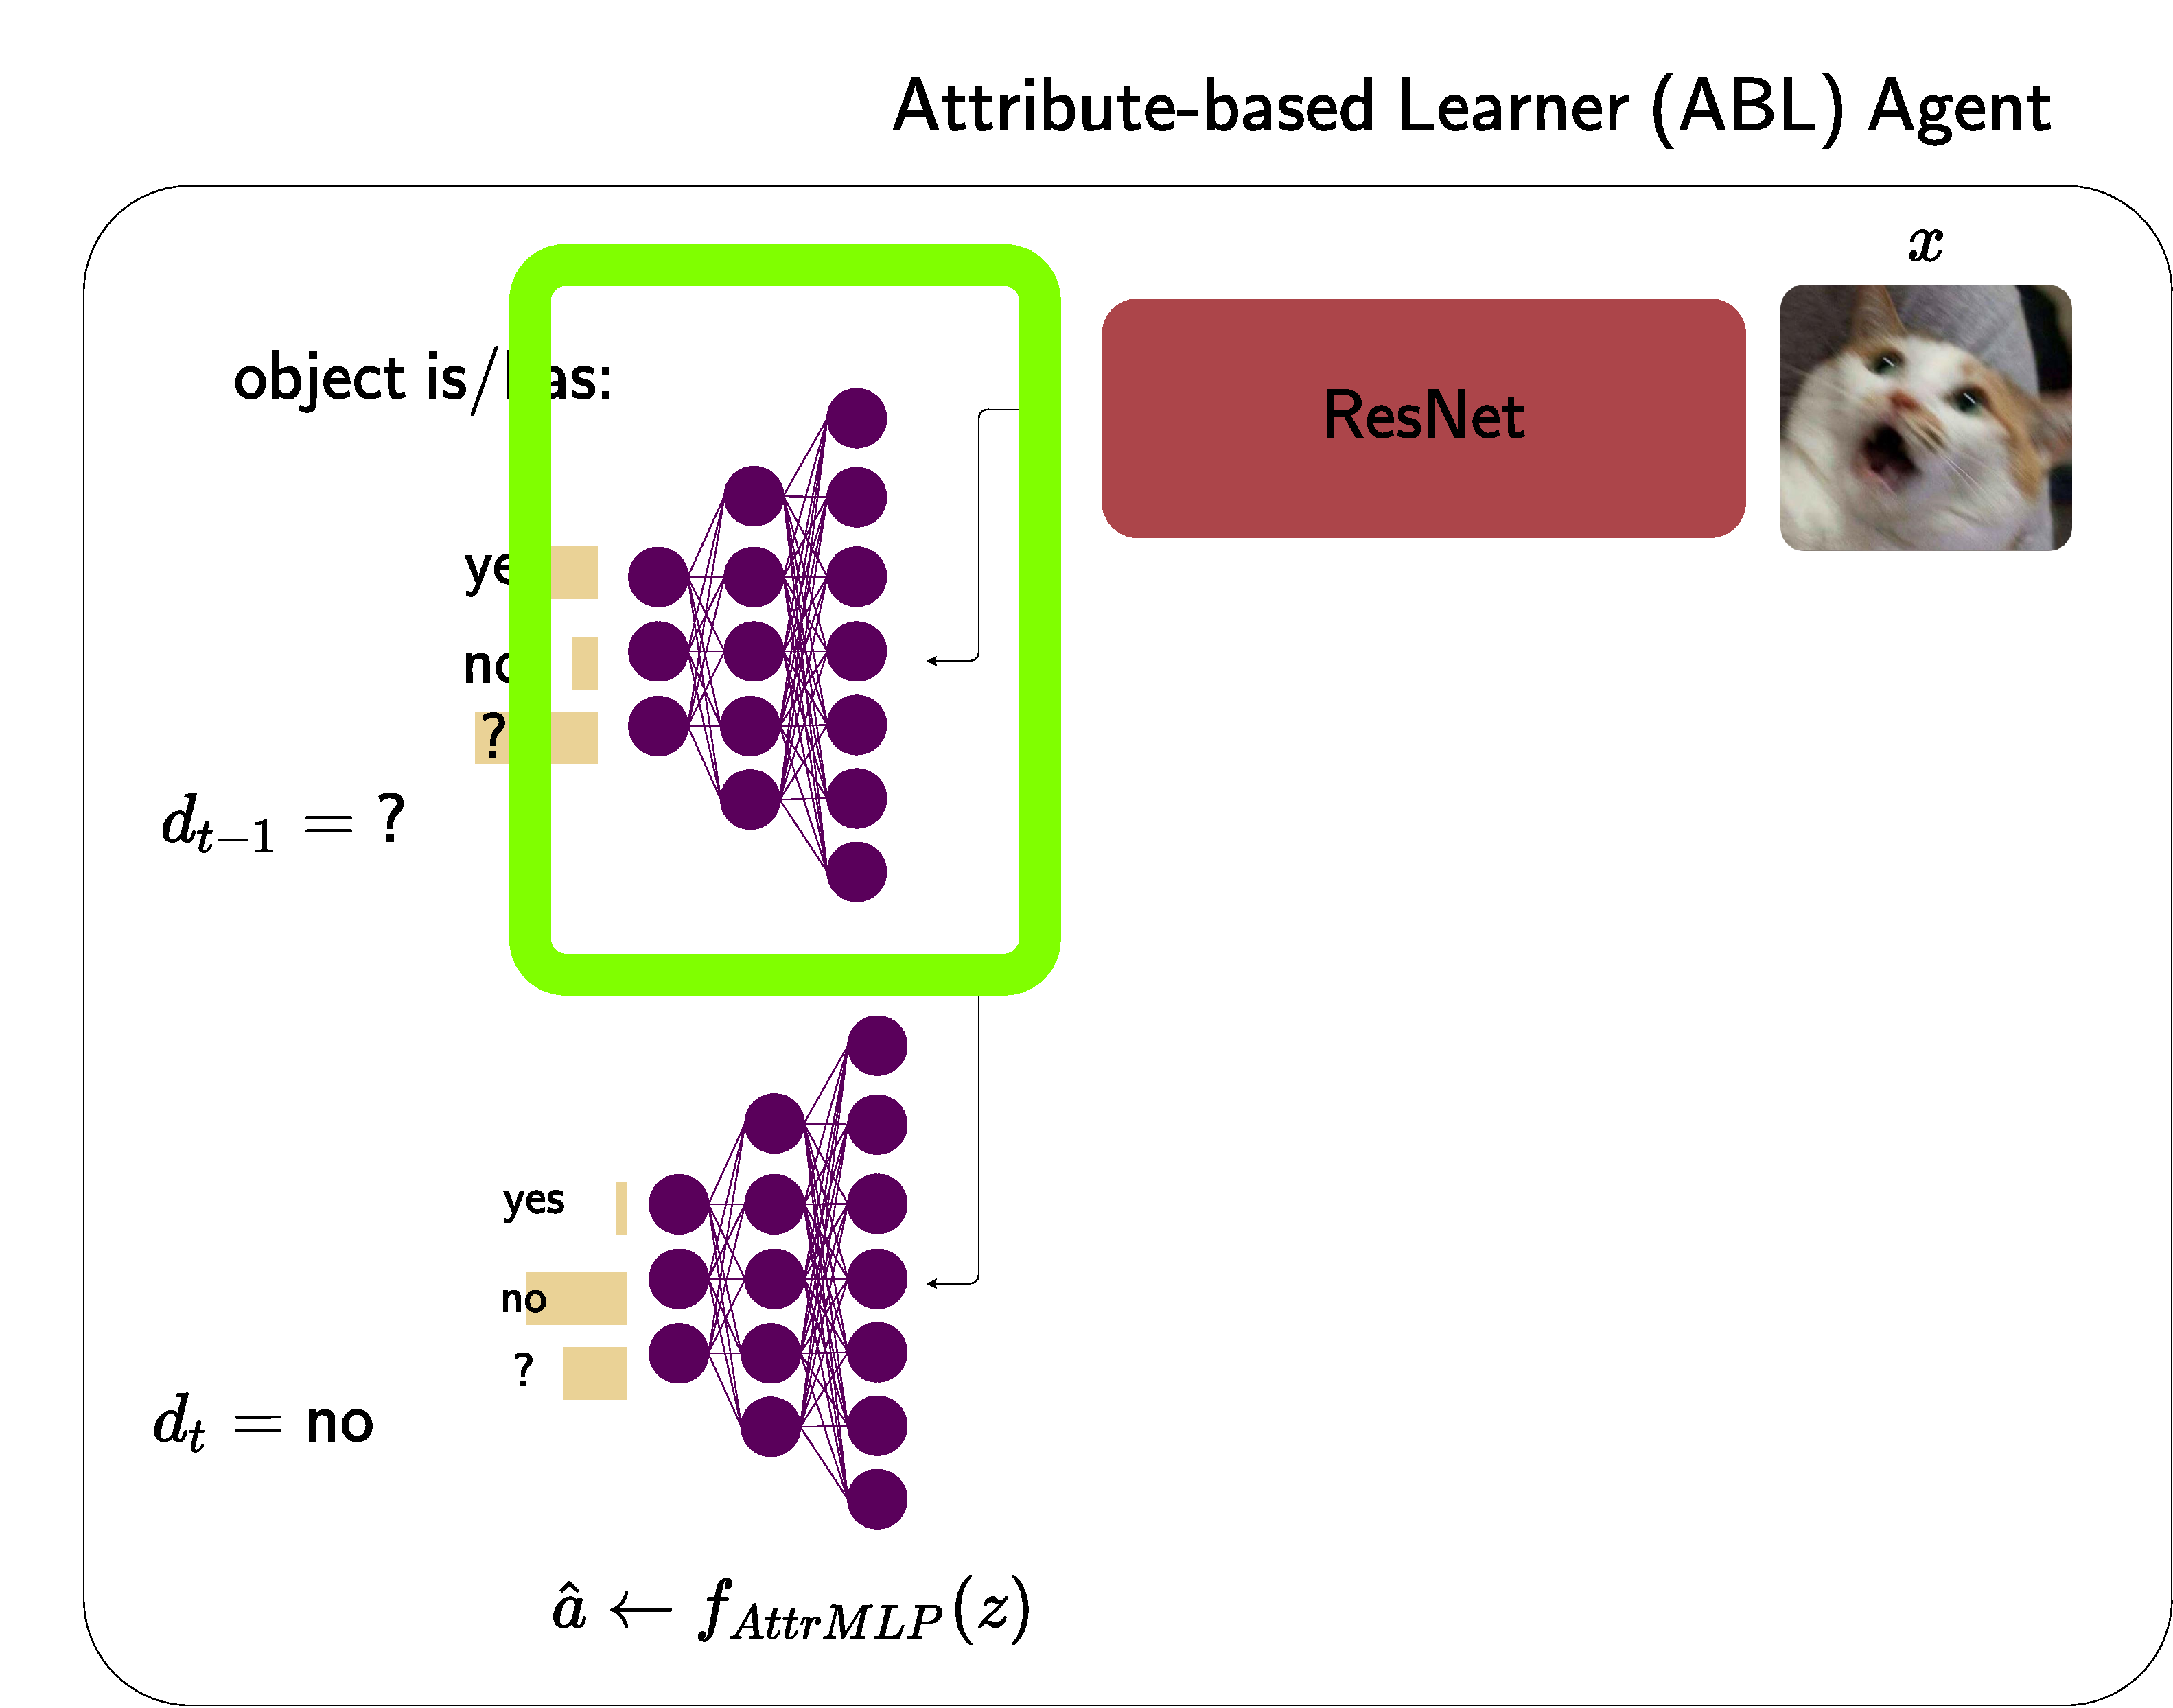
\includegraphics[width=\textwidth]{images/urdtc_parts_attrMLP.pdf}
\end{column}
\end{columns}
\end{frame}

\setbeamercolor{background canvas}{bg=white}
\setbeamercolor{normal text}{fg=darkgrey}
\usebeamercolor[fg]{normal text}
\setbeamertemplate{itemize item}{\color{darkgrey}$\circ$}
\begin{frame}
\frametitle{Recurrent Decision Tree}
\framesubtitle{LSTM}
\begin{columns}[T]
\begin{column}{.5\textwidth}
\begin{itemize}
	% Your text here
	\item Hidden state based on answers
	\item and explicit memory
	\item Basis for next question
	\item Basis for classification
\end{itemize}
\end{column}
\begin{column}{.5\textwidth}
% Your image included here
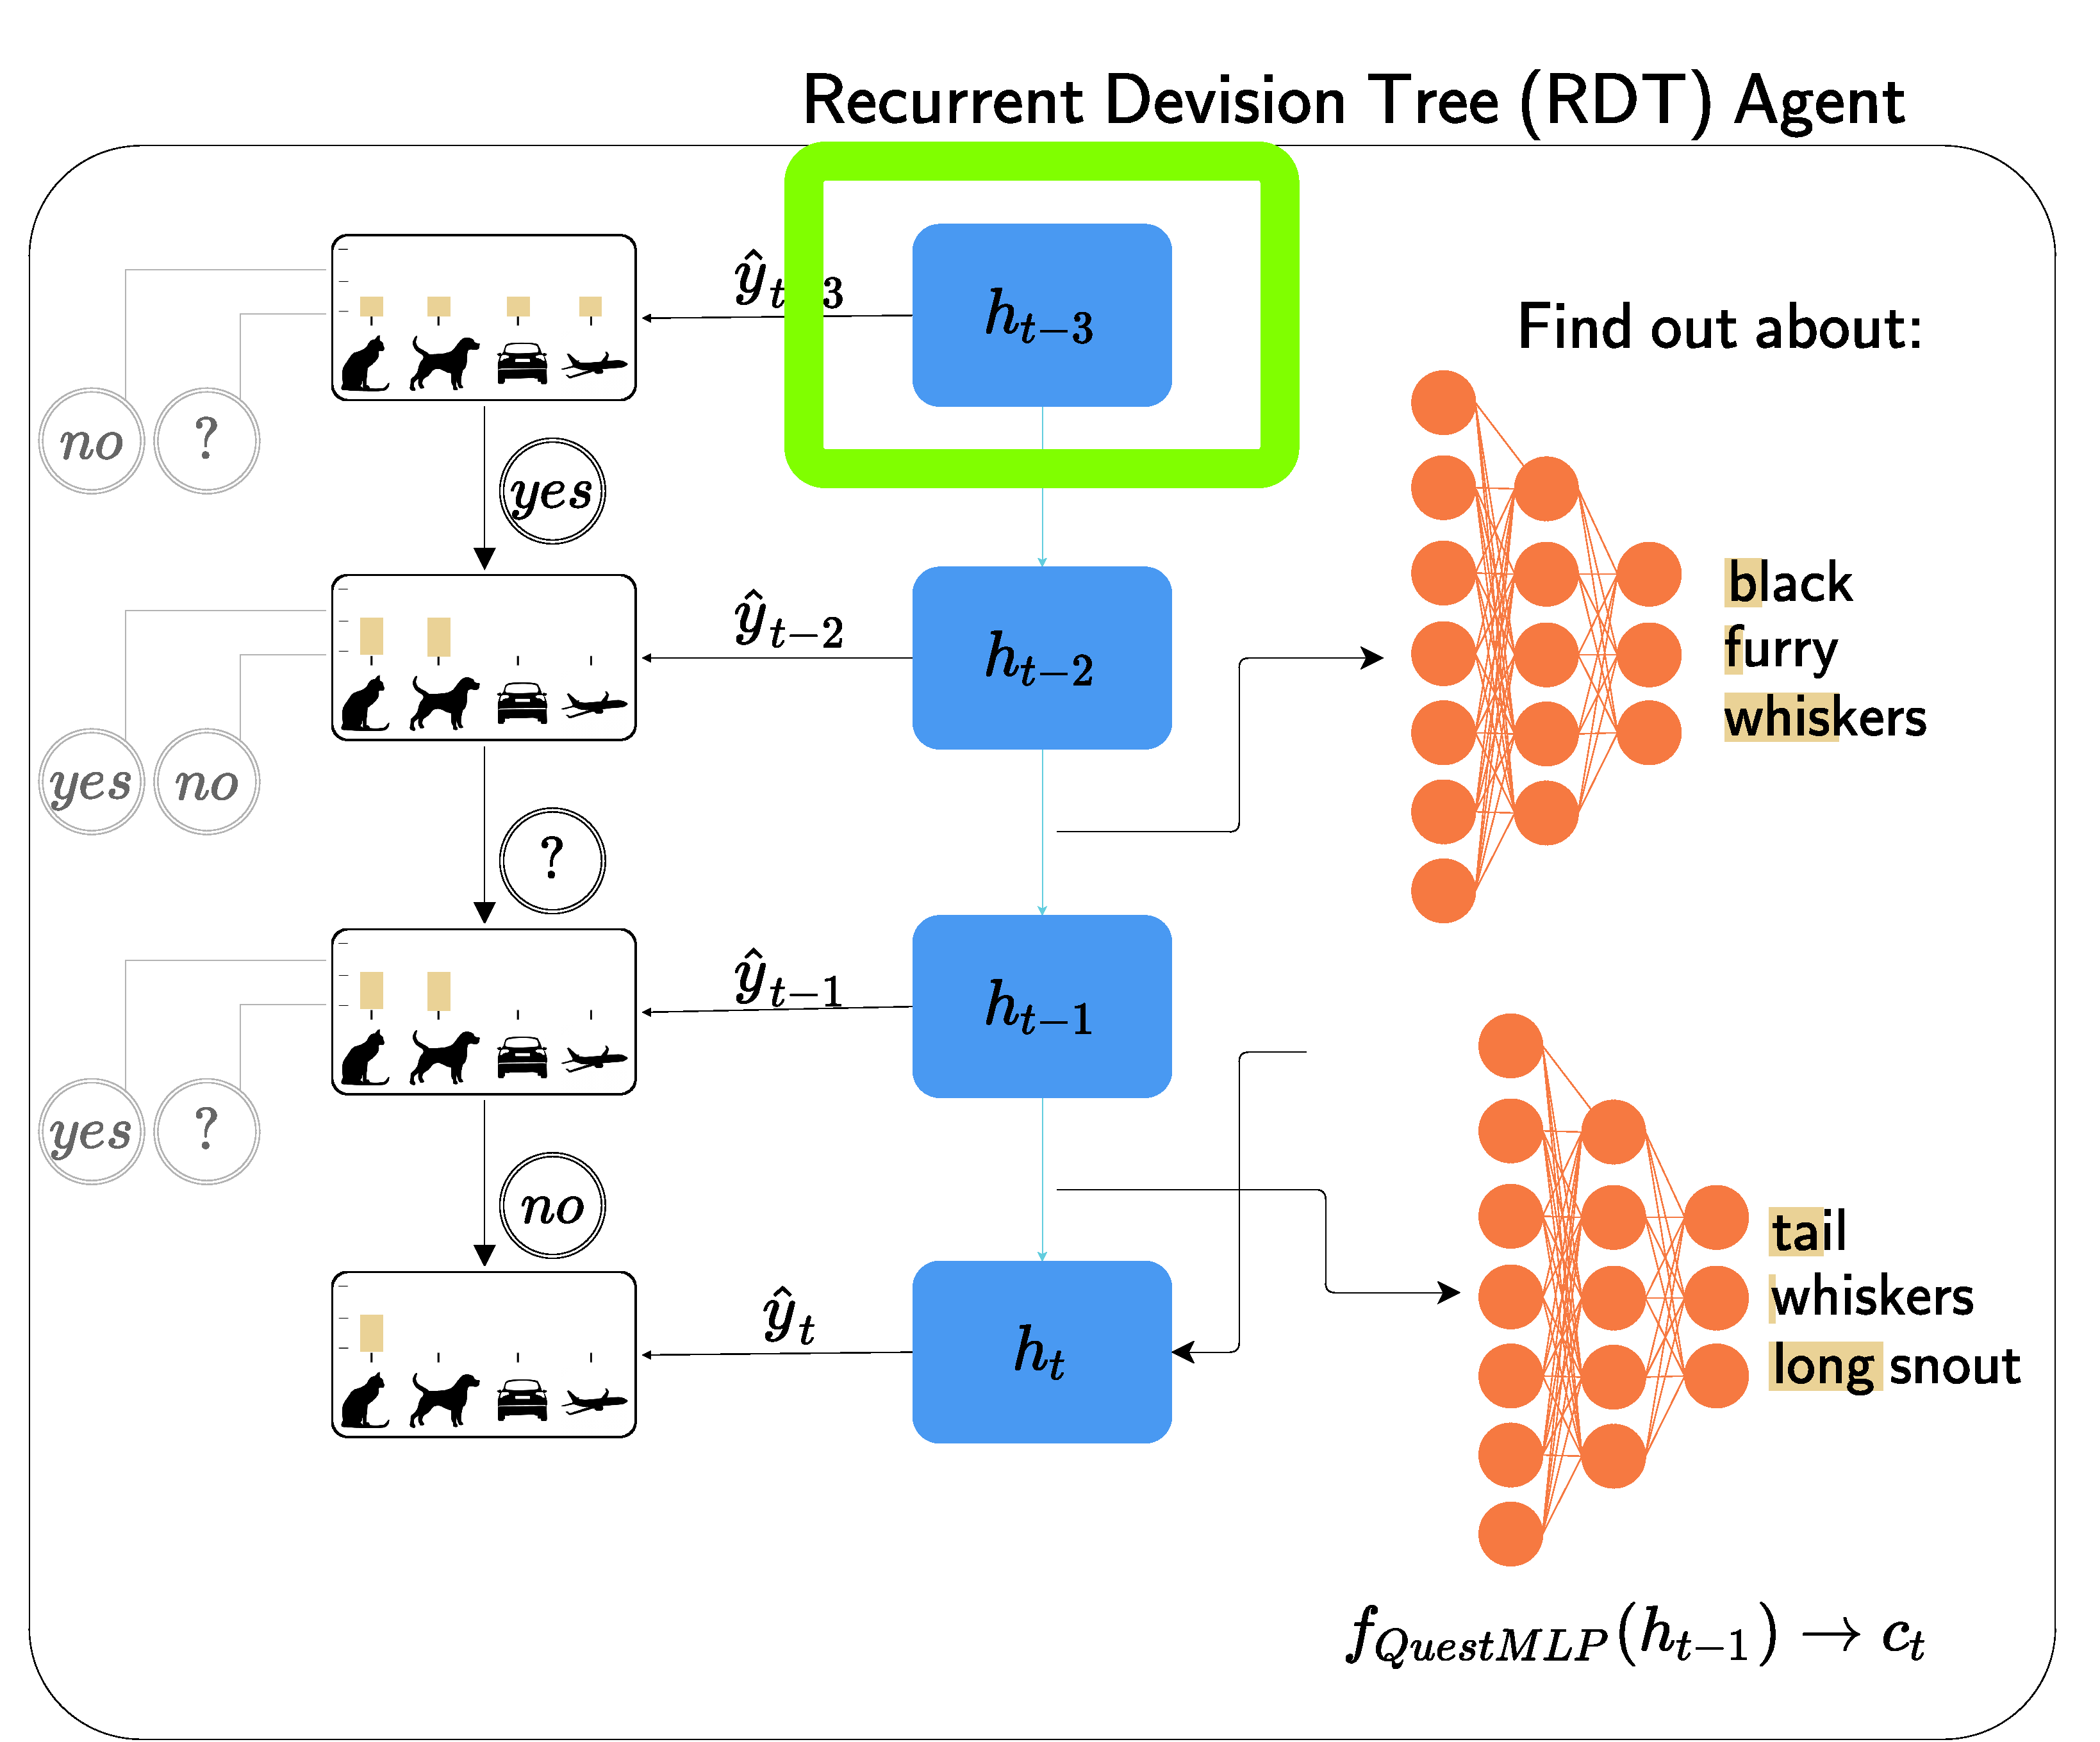
\includegraphics[width=\textwidth]{images/urdtc_parts_lstm.pdf}
\end{column}
\end{columns}
\end{frame}

\setbeamercolor{background canvas}{bg=white}
\setbeamercolor{normal text}{fg=darkgrey}
\usebeamercolor[fg]{normal text}
\setbeamertemplate{itemize item}{\color{darkgrey}$\circ$}
\begin{frame}
\frametitle{Recurrent Decision Tree}
\framesubtitle{Choosing questions}
\begin{columns}[T]
\begin{column}{.5\textwidth}
\begin{itemize}
% Your text here
	\item Pose new question
	\item based on LSTM
	\item $c_t \sim p(c_t)$
	\item GumbelSoftmax
	\item Sample from categorical distribution
	\item $d_t = \hat{a}\left[c_t\right]$
\end{itemize}
\end{column}
\begin{column}{.5\textwidth}
% Your image included here
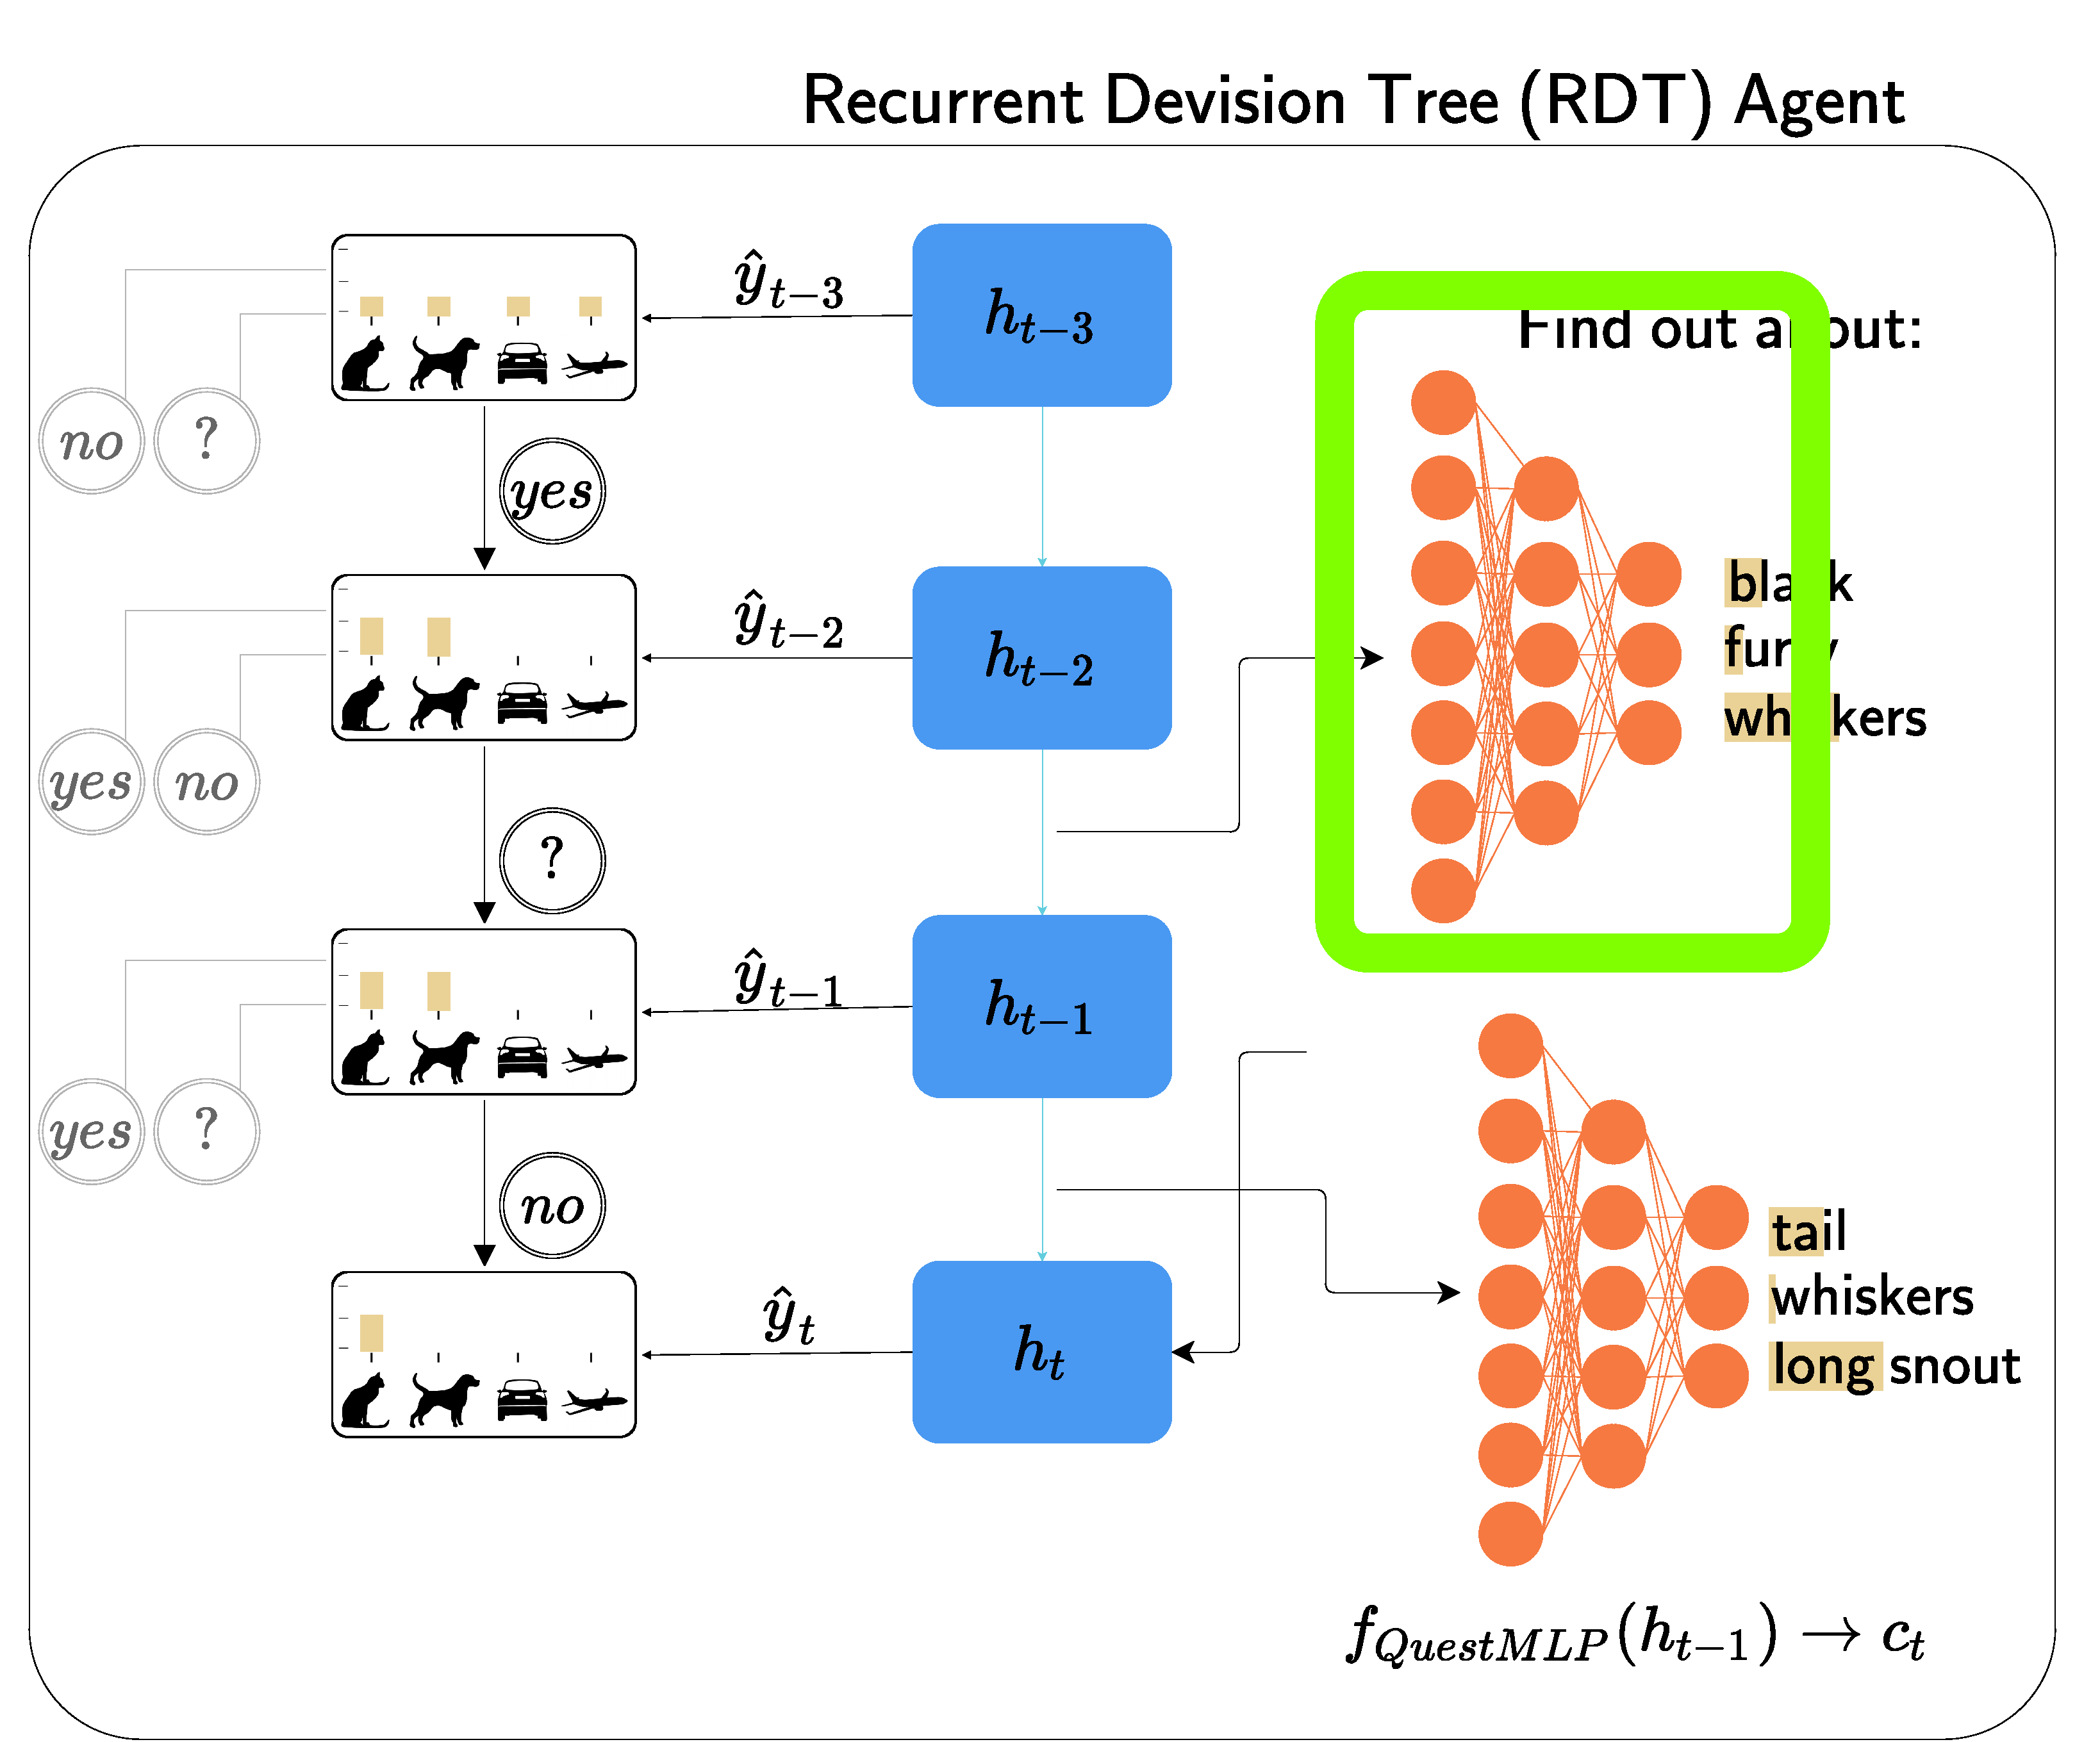
\includegraphics[width=\textwidth]{images/urdtc_parts_questMLP.pdf}
\end{column}
\end{columns}
\end{frame}

\setbeamercolor{background canvas}{bg=white}
\setbeamercolor{normal text}{fg=darkgrey}
\usebeamercolor[fg]{normal text}
\setbeamertemplate{itemize item}{\color{darkgrey}$\circ$}
\begin{frame}
\frametitle{Recurrent Decision Tree}
\framesubtitle{Making a classification}
\begin{columns}[T]
\begin{column}{.5\textwidth}
\begin{itemize}
	\item Classification in each communication step
	\item For classification loss
\end{itemize}
\end{column}
\begin{column}{.5\textwidth}
% Your image included here
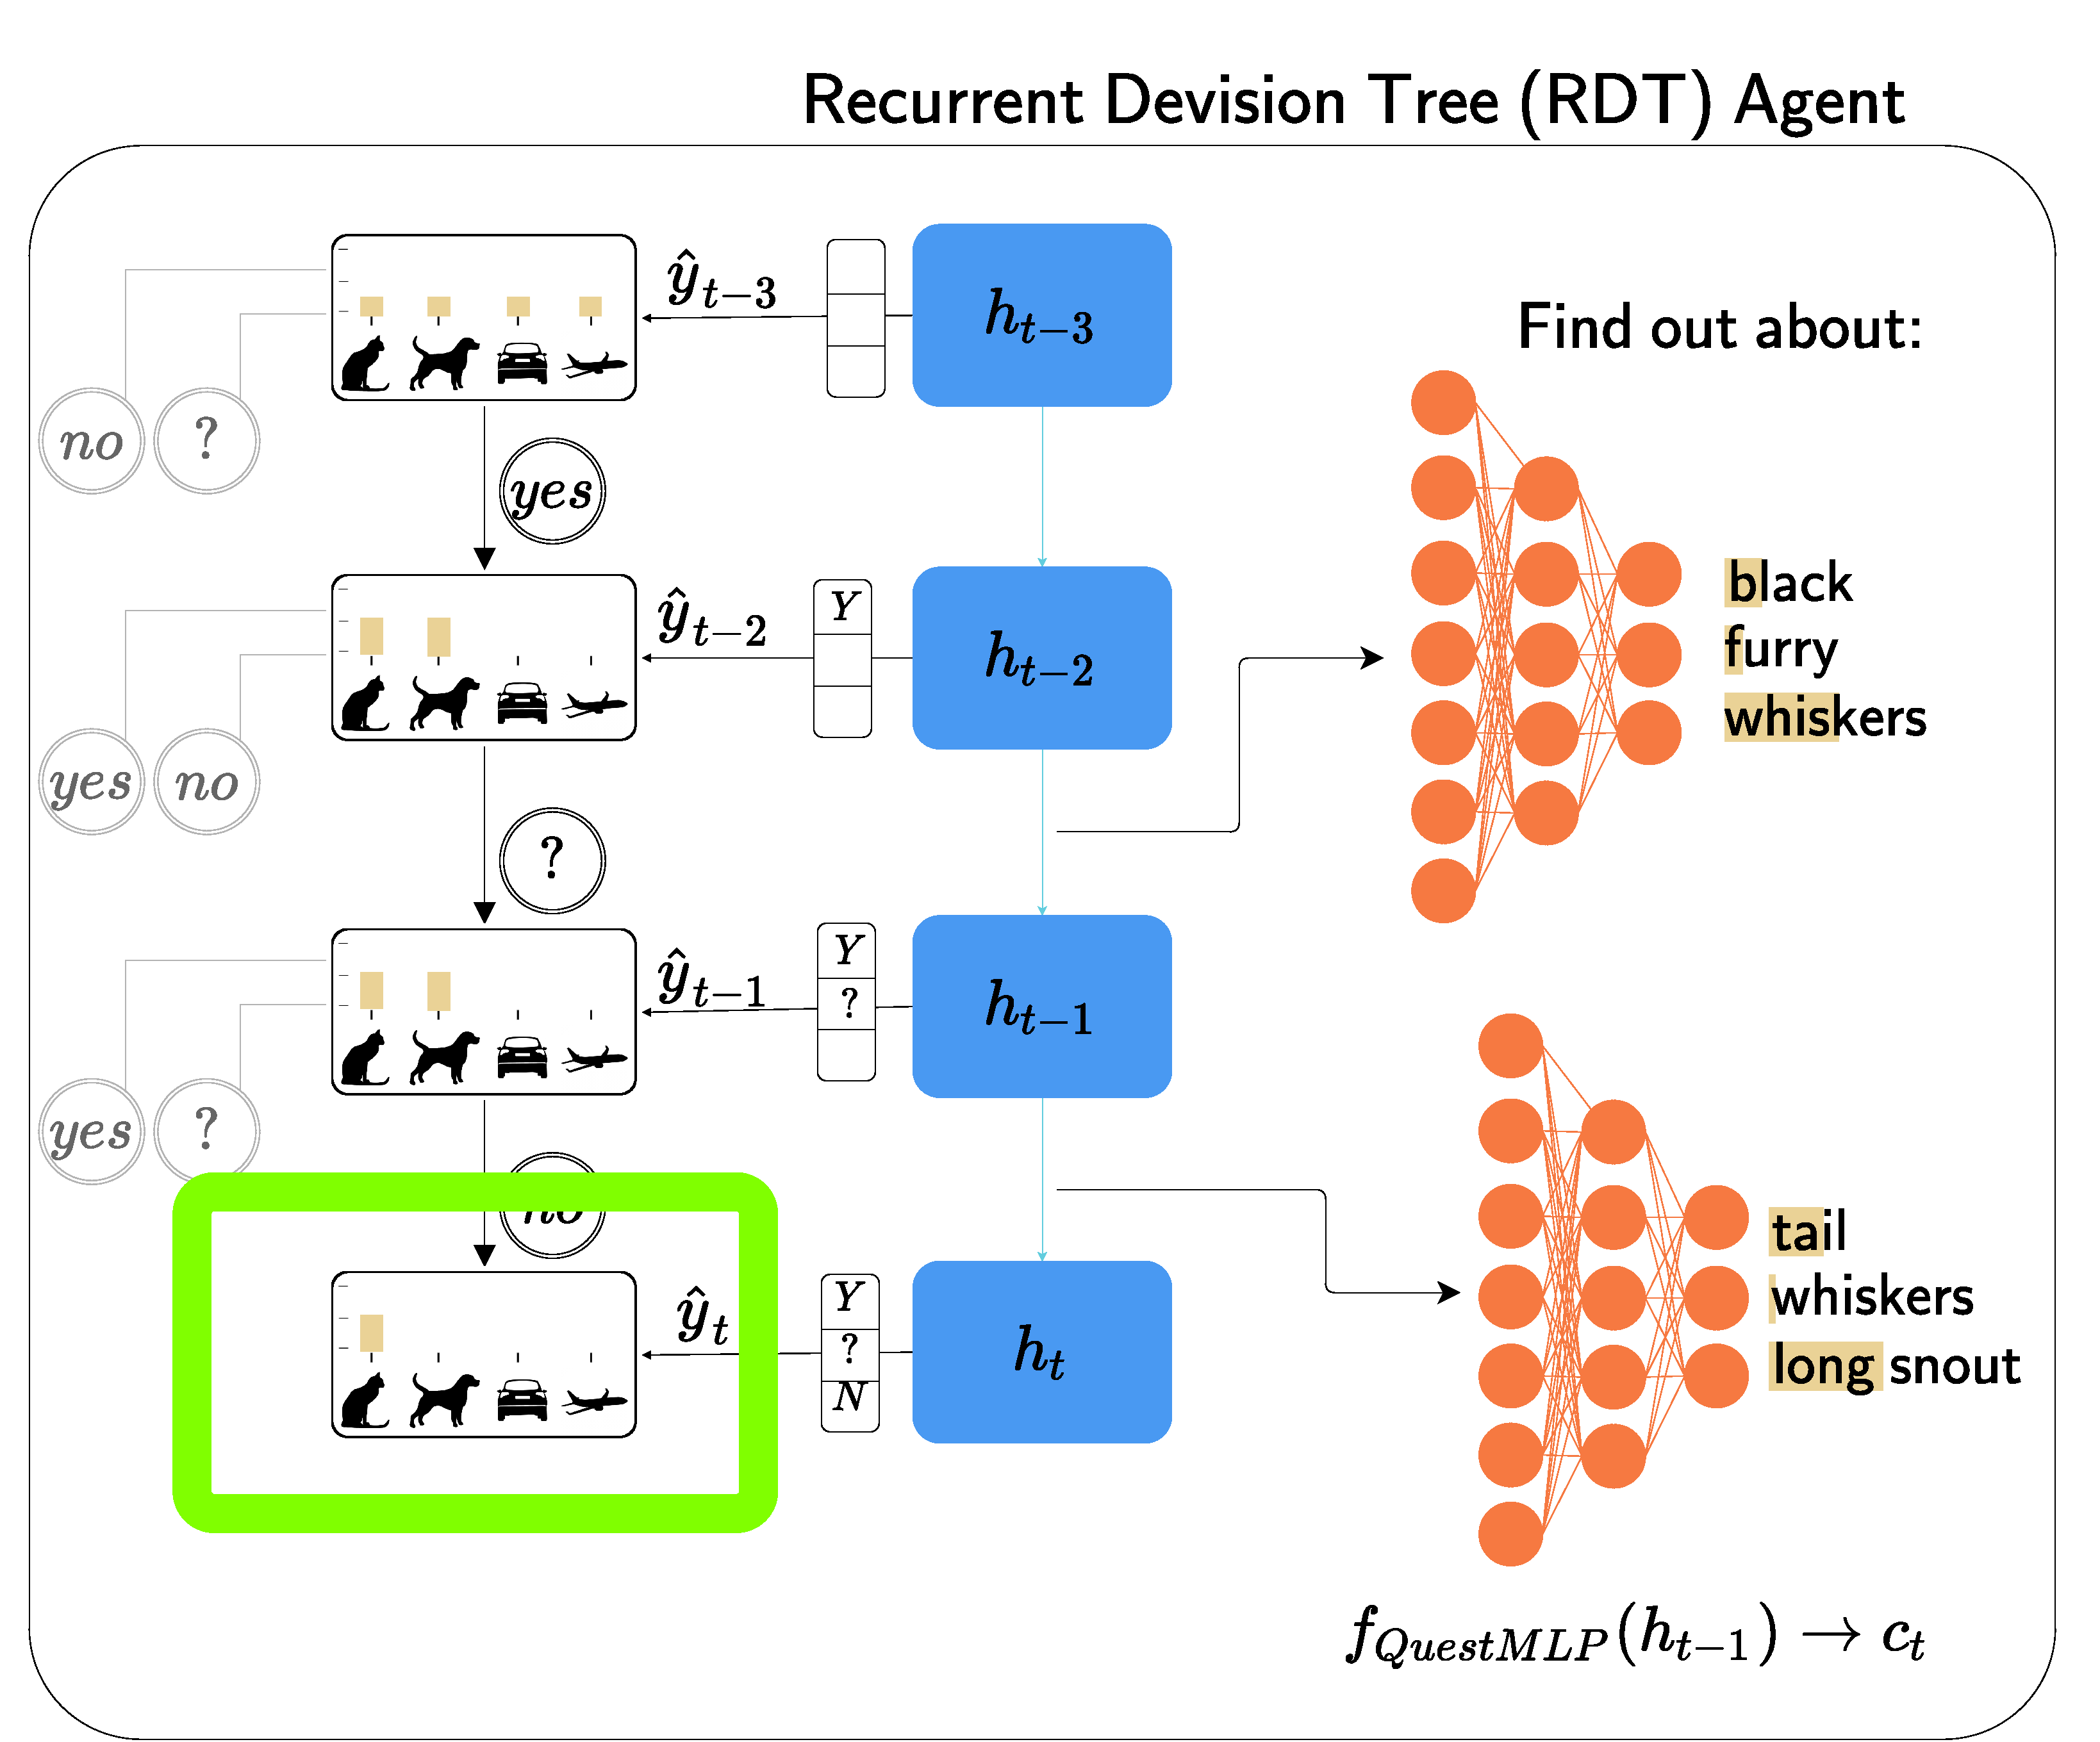
\includegraphics[width=\textwidth]{images/urdtc_parts_classMLP.pdf}
\end{column}
\end{columns}
\end{frame}

% Trianing
\setbeamercolor{background canvas}{bg=white}
\setbeamercolor{normal text}{fg=darkgrey}
\usebeamercolor[fg]{normal text}
\setbeamertemplate{itemize item}{\color{darkgrey}$\circ$}	
\begin{frame}
\frametitle{Training}
\framesubtitle{Joint Objective}
\begin{itemize}
	\item Optimize for class (and attribute accuracy)
	\begin{align*}
	\mathcal{L} = \frac{1}{T}\sum_{t=1}^{T}\left[(1-\lambda)\mathcal{L}_{CE}(y,\hat{y}_t) + \lambda \mathcal{L}_{CE}(\alpha_{y,c_t},\hat{\alpha}_{c_t}) \right]
	\end{align*}
	\item $\lambda$ can be used to balance the two loss terms
	\item For all of our experiments, we use $\lambda=0.2$
	\item Discourage deep trees%with $T$ %(number of communication steps)
\end{itemize}
\end{frame}



\setbeamercolor{background canvas}{bg=orange}
\setbeamercolor{normal text}{fg=white}	
\usebeamercolor[fg]{normal text}
\setbeamertemplate{itemize item}{\color{white}$\circ$}
\begin{frame}
\frametitle{The RDTC Model \cite{alaniz2019explainable}}
\begin{itemize}
	%\item RDTC is a model consisting of two agents
	\item AbL can see data, and answer all questions in advance
	\item RDT can choose attributes to question
	\item Get answer through indexing
	\item Joint objective of maximizing class and attribute accuracy
\end{itemize}
\end{frame}
%\setbeamertemplate{background canvas}{bg=default}







% Related Work
\setbeamercolor{background canvas}{bg=white}
\setbeamercolor{normal text}{fg=darkgrey}
\usebeamercolor[fg]{normal text}
\setbeamertemplate{itemize item}{\color{darkgrey}$\circ$}	
\begin{frame}
\frametitle{Background}
\framesubtitle{A small excursion to Gaussian Processes (GP)}
\begin{figure}
	\centering
	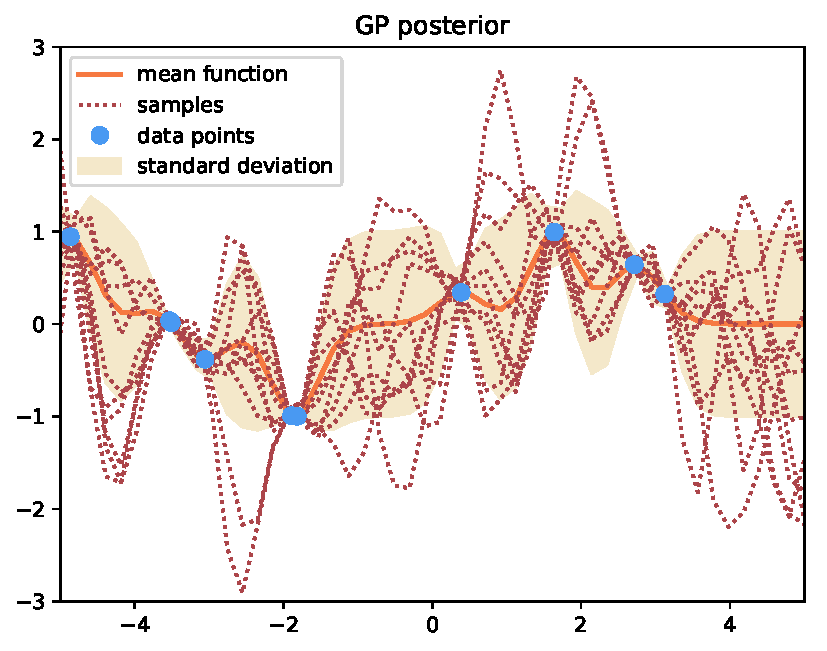
\includegraphics[width=0.6\textwidth]{images/post.pdf}
	\begin{itemize}
		\item Data can be described by (infinitely) many functions
		\item A GP is a PDF over these functions
		\item Intuition: $\rightarrow$ GP yields probability for function values %at any index
		\item Parameterized by mean function and covariance function
		\item Variance corresponds to model uncertainty
	\end{itemize}
	%\caption{Correlations between misclassification rate, uncertainty, and usage of attributes.}
	%\label{fig:corr_matrix}
\end{figure}
\end{frame}


\begin{frame}
\setbeamercolor{background canvas}{bg=white}
\setbeamercolor{normal text}{fg=darkgrey}
\usebeamercolor[fg]{normal text}
\setbeamertemplate{itemize item}{\color{darkgrey}$\circ$}	
\frametitle{Background}
\framesubtitle{Dropout Uncertainty Estimation}
	\begin{itemize}
	%\item A GP can be seen as an infinitely wide neural network
	\item Gal and Ghahramani \cite{gal2016dropout} proof that variance from dropout corresponds to model uncertainty
	\item We use their proof as foundation for our uncertainty estimate
	%\item Key idea is to rewrite objective of Variational GP as dropout neural net objective
	\item Neural net is set of weighted linear functions, activated by non-linearity
	\item Putting PDF over each weight creates finite GP
\end{itemize}
\end{frame}

\begin{frame}
\setbeamercolor{background canvas}{bg=white}
\setbeamercolor{normal text}{fg=darkgrey}
\usebeamercolor[fg]{normal text}
\setbeamertemplate{itemize item}{\color{darkgrey}$\circ$}	
\frametitle{Background}
\framesubtitle{Dropout Uncertainty Estimation}
\begin{itemize}
	%\item A GP can be seen as an infinitely wide neural network
	\item We can view neural net as approximation to GP
	%\item In turn, we can view a neural network with a finite amount of units as an approximation to a GP
	\item Posterior over functions requires computing integrals
	\item Intractable integrals require methods of variational inference
	\begin{itemize}
		\item GP objective $\rightarrow$ minimization objective
		\item For covariance function $\rightarrow$ Monte-Carlo integration
	\end{itemize}
	\item Variational GP's objective can be rewritten as dropout net
	%\item This allows us to rewrite a GP's objective as to objective of a dropout neural network
	\item Variance arising from dropout can be interpreted as model uncertainty
\end{itemize}
\end{frame}




\setbeamercolor{background canvas}{bg=white}
\setbeamercolor{normal text}{fg=darkgrey}
\usebeamercolor[fg]{normal text}
\setbeamertemplate{itemize item}{\color{darkgrey}$\circ$}
\begin{frame}
\frametitle{How?}
\framesubtitle{How do we get uncertainty information?}\begin{figure}
	\centering
	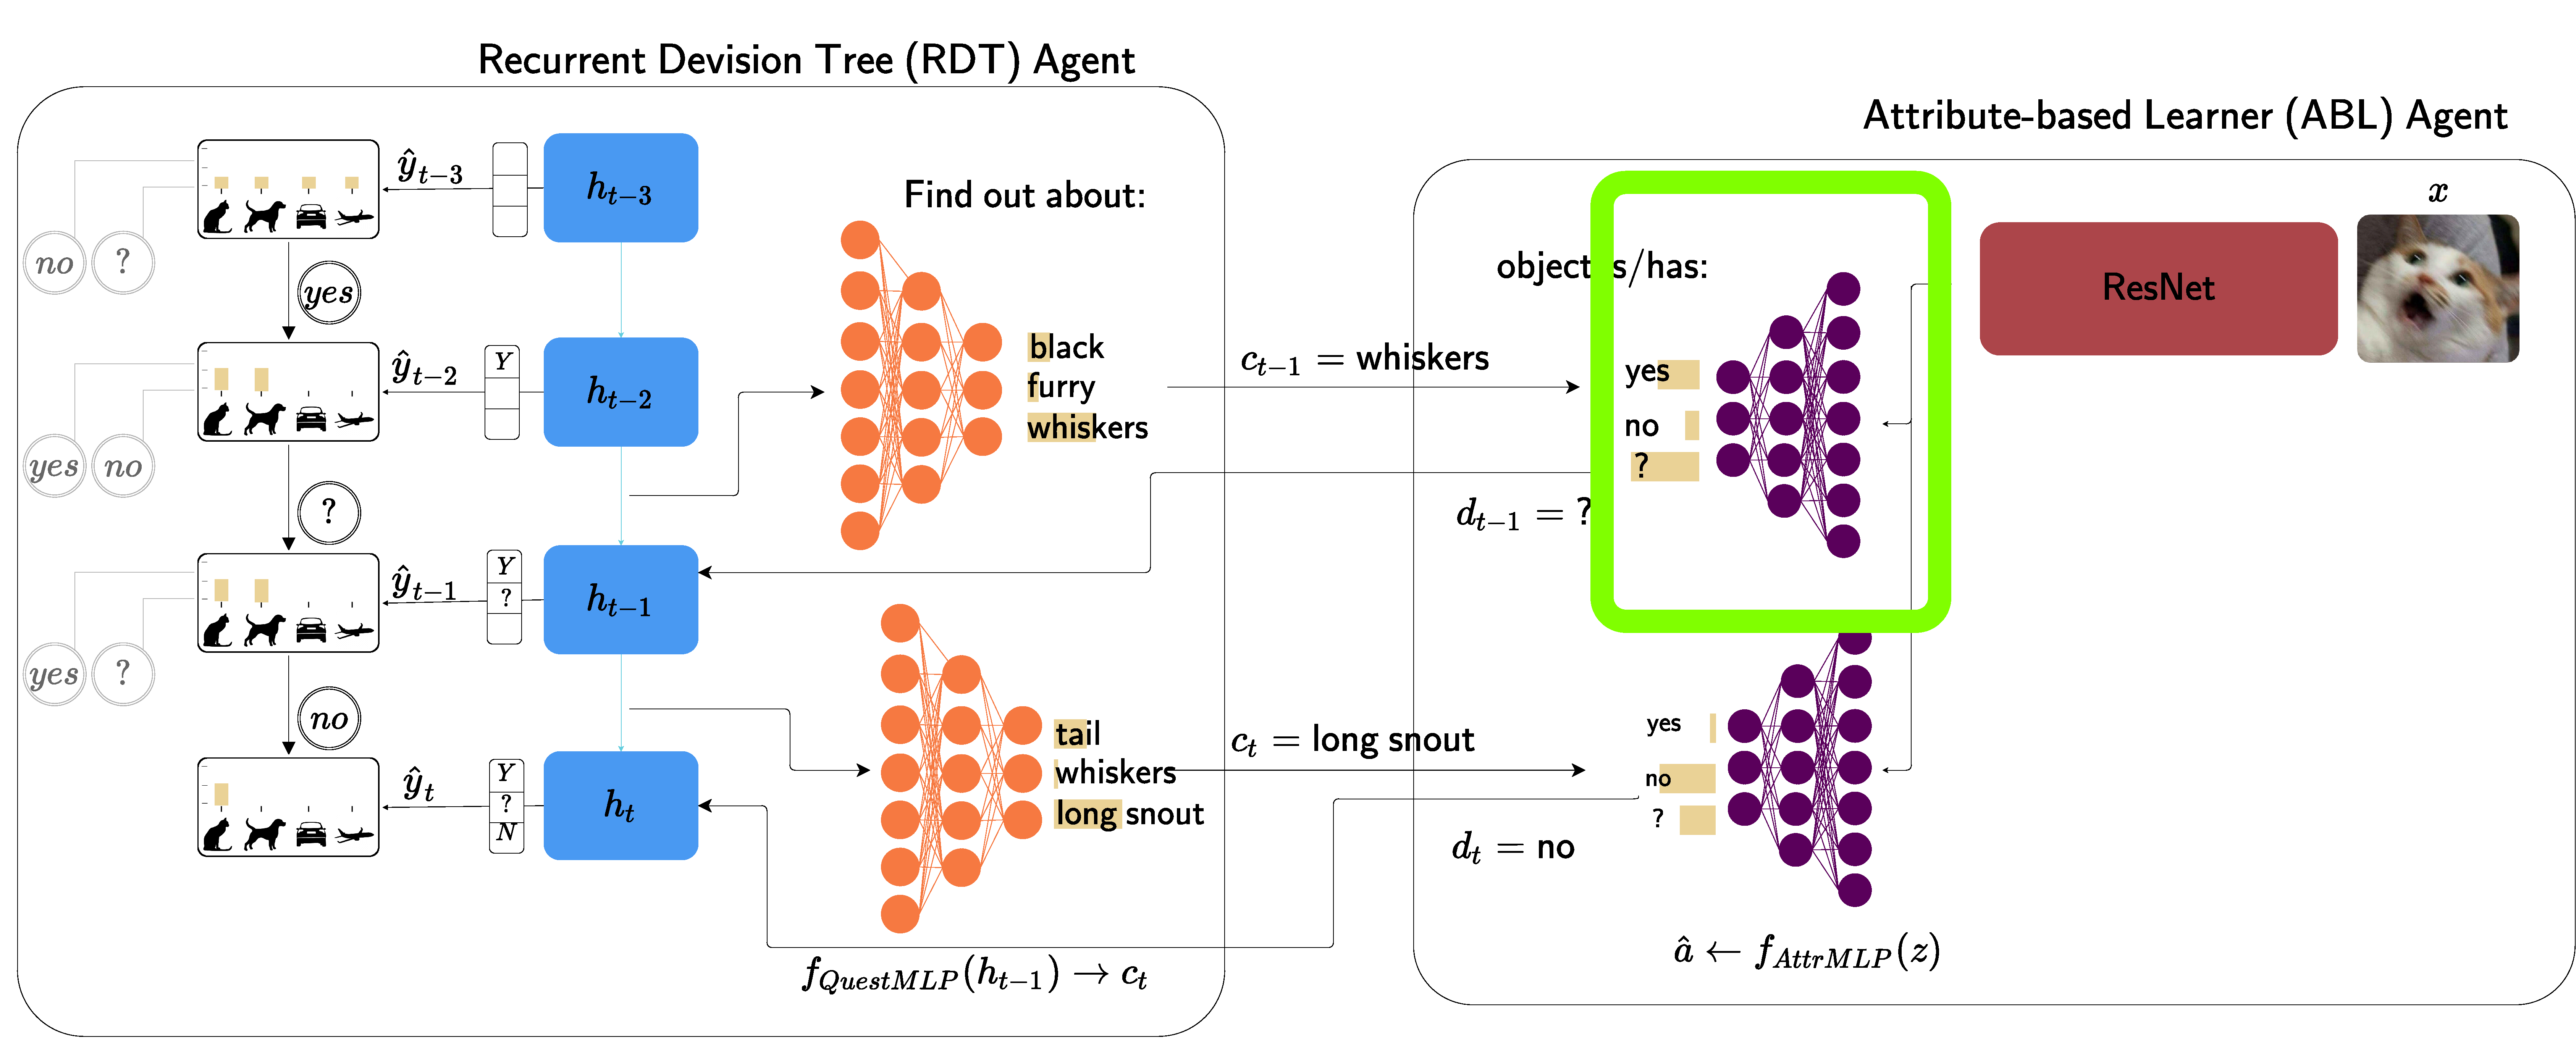
\includegraphics[width=0.8\textwidth]{images/where_is_uncertainty.pdf} 
\end{figure}
\begin{itemize}
	\item We use Gal and Ghahramani's \cite{gal2016dropout} proof to estimate uncertainty 
	\item We want AbL to say '?' in the case of high uncertainty
	%\item However, we want to keep the ResNet as feature extractor
	\item Make $f_{AttrMLP}$ a dropout MLP
	\item After extracting features $\rightarrow$ compute $Var(n \;forward\;passes)$
	\item According to proof, this corresponds to model uncertainty
\end{itemize}
\end{frame}



%%%%%%%%%%%%%%%%%%%%%%%%%%%%%%%%%%%%%%%%%%%%%%%%%%%%%%%%



%%%%%%%%%%%%%%%%%%%%%%%%%%%%%%%%%%%%%%%%%%%%%%%%%%%%%













\setbeamercolor{background canvas}{bg=white}
\setbeamercolor{normal text}{fg=darkgrey}
\usebeamercolor[fg]{normal text}
\setbeamertemplate{itemize item}{\color{darkgrey}$\circ$}	
\begin{frame}
\frametitle{Getting Uncertainty Information}
\framesubtitle{Estimating Uncertainty in the AbL}
\begin{figure}
	\centering
	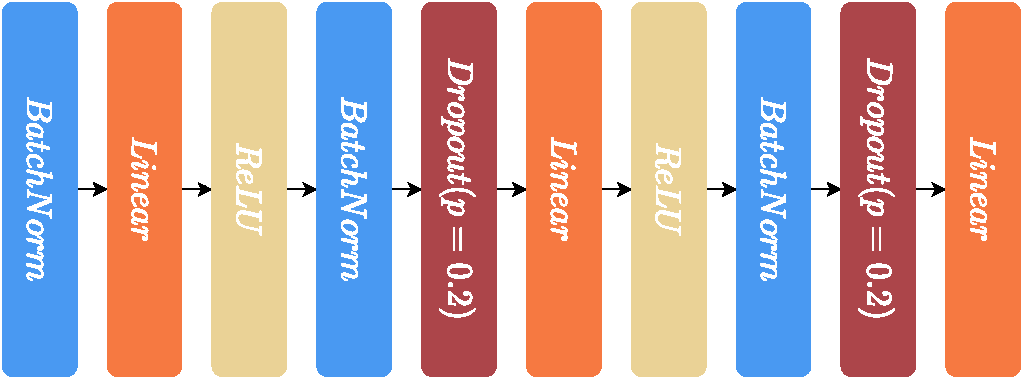
\includegraphics[width=0.7\textwidth]{images/f_attrMLP.pdf}
\end{figure}
\begin{itemize}
	\item We include dropout layers in $f_{AttrMLP}$
	\item We tested different configurations
	\item Combination of batchnorm and dropout worked best
\end{itemize}
\end{frame}



\setbeamercolor{background canvas}{fg=darkgrey}
\setbeamercolor{normal text}{fg=darkgrey}
\usebeamercolor[fg]{normal text}
\setbeamertemplate{itemize item}{\color{darkgrey}$\circ$}
\begin{frame}	
\frametitle{Using Uncertainty Information}
\framesubtitle{Uncertainty Information as Inductive Bias}
\begin{itemize}
	%\item Now, we have an uncertainty estimate
	%\item But now, we need a way to use it
	\item We use uncertainty in two different strategies
	\begin{itemize}
		\item Prevent model from asking about uncertain attributes\\$\rightarrow$ remRDTC
		\item We give the model the ability to answer with 'I don't know'\\$\rightarrow$ extRDTC
	\end{itemize}
	\item Don't allow the model to use gradients from uncertain attributes
	\item Uncertainty information remains inductive bias% and can not be misused
	%\item This ensures that the uncertainty information only serves as an inductive bias and the model does not misuse it
\end{itemize}
\end{frame}


\setbeamercolor{background canvas}{bg=white}	
\setbeamercolor{normal text}{fg=darkgrey}
\usebeamercolor[fg]{normal text}
\setbeamertemplate{itemize item}{\color{darkgrey}$\circ$}
\begin{frame}
\frametitle{Using Uncertainty Information}
\framesubtitle{Removing uncertain attributes (remRDTC)}
\begin{figure}
	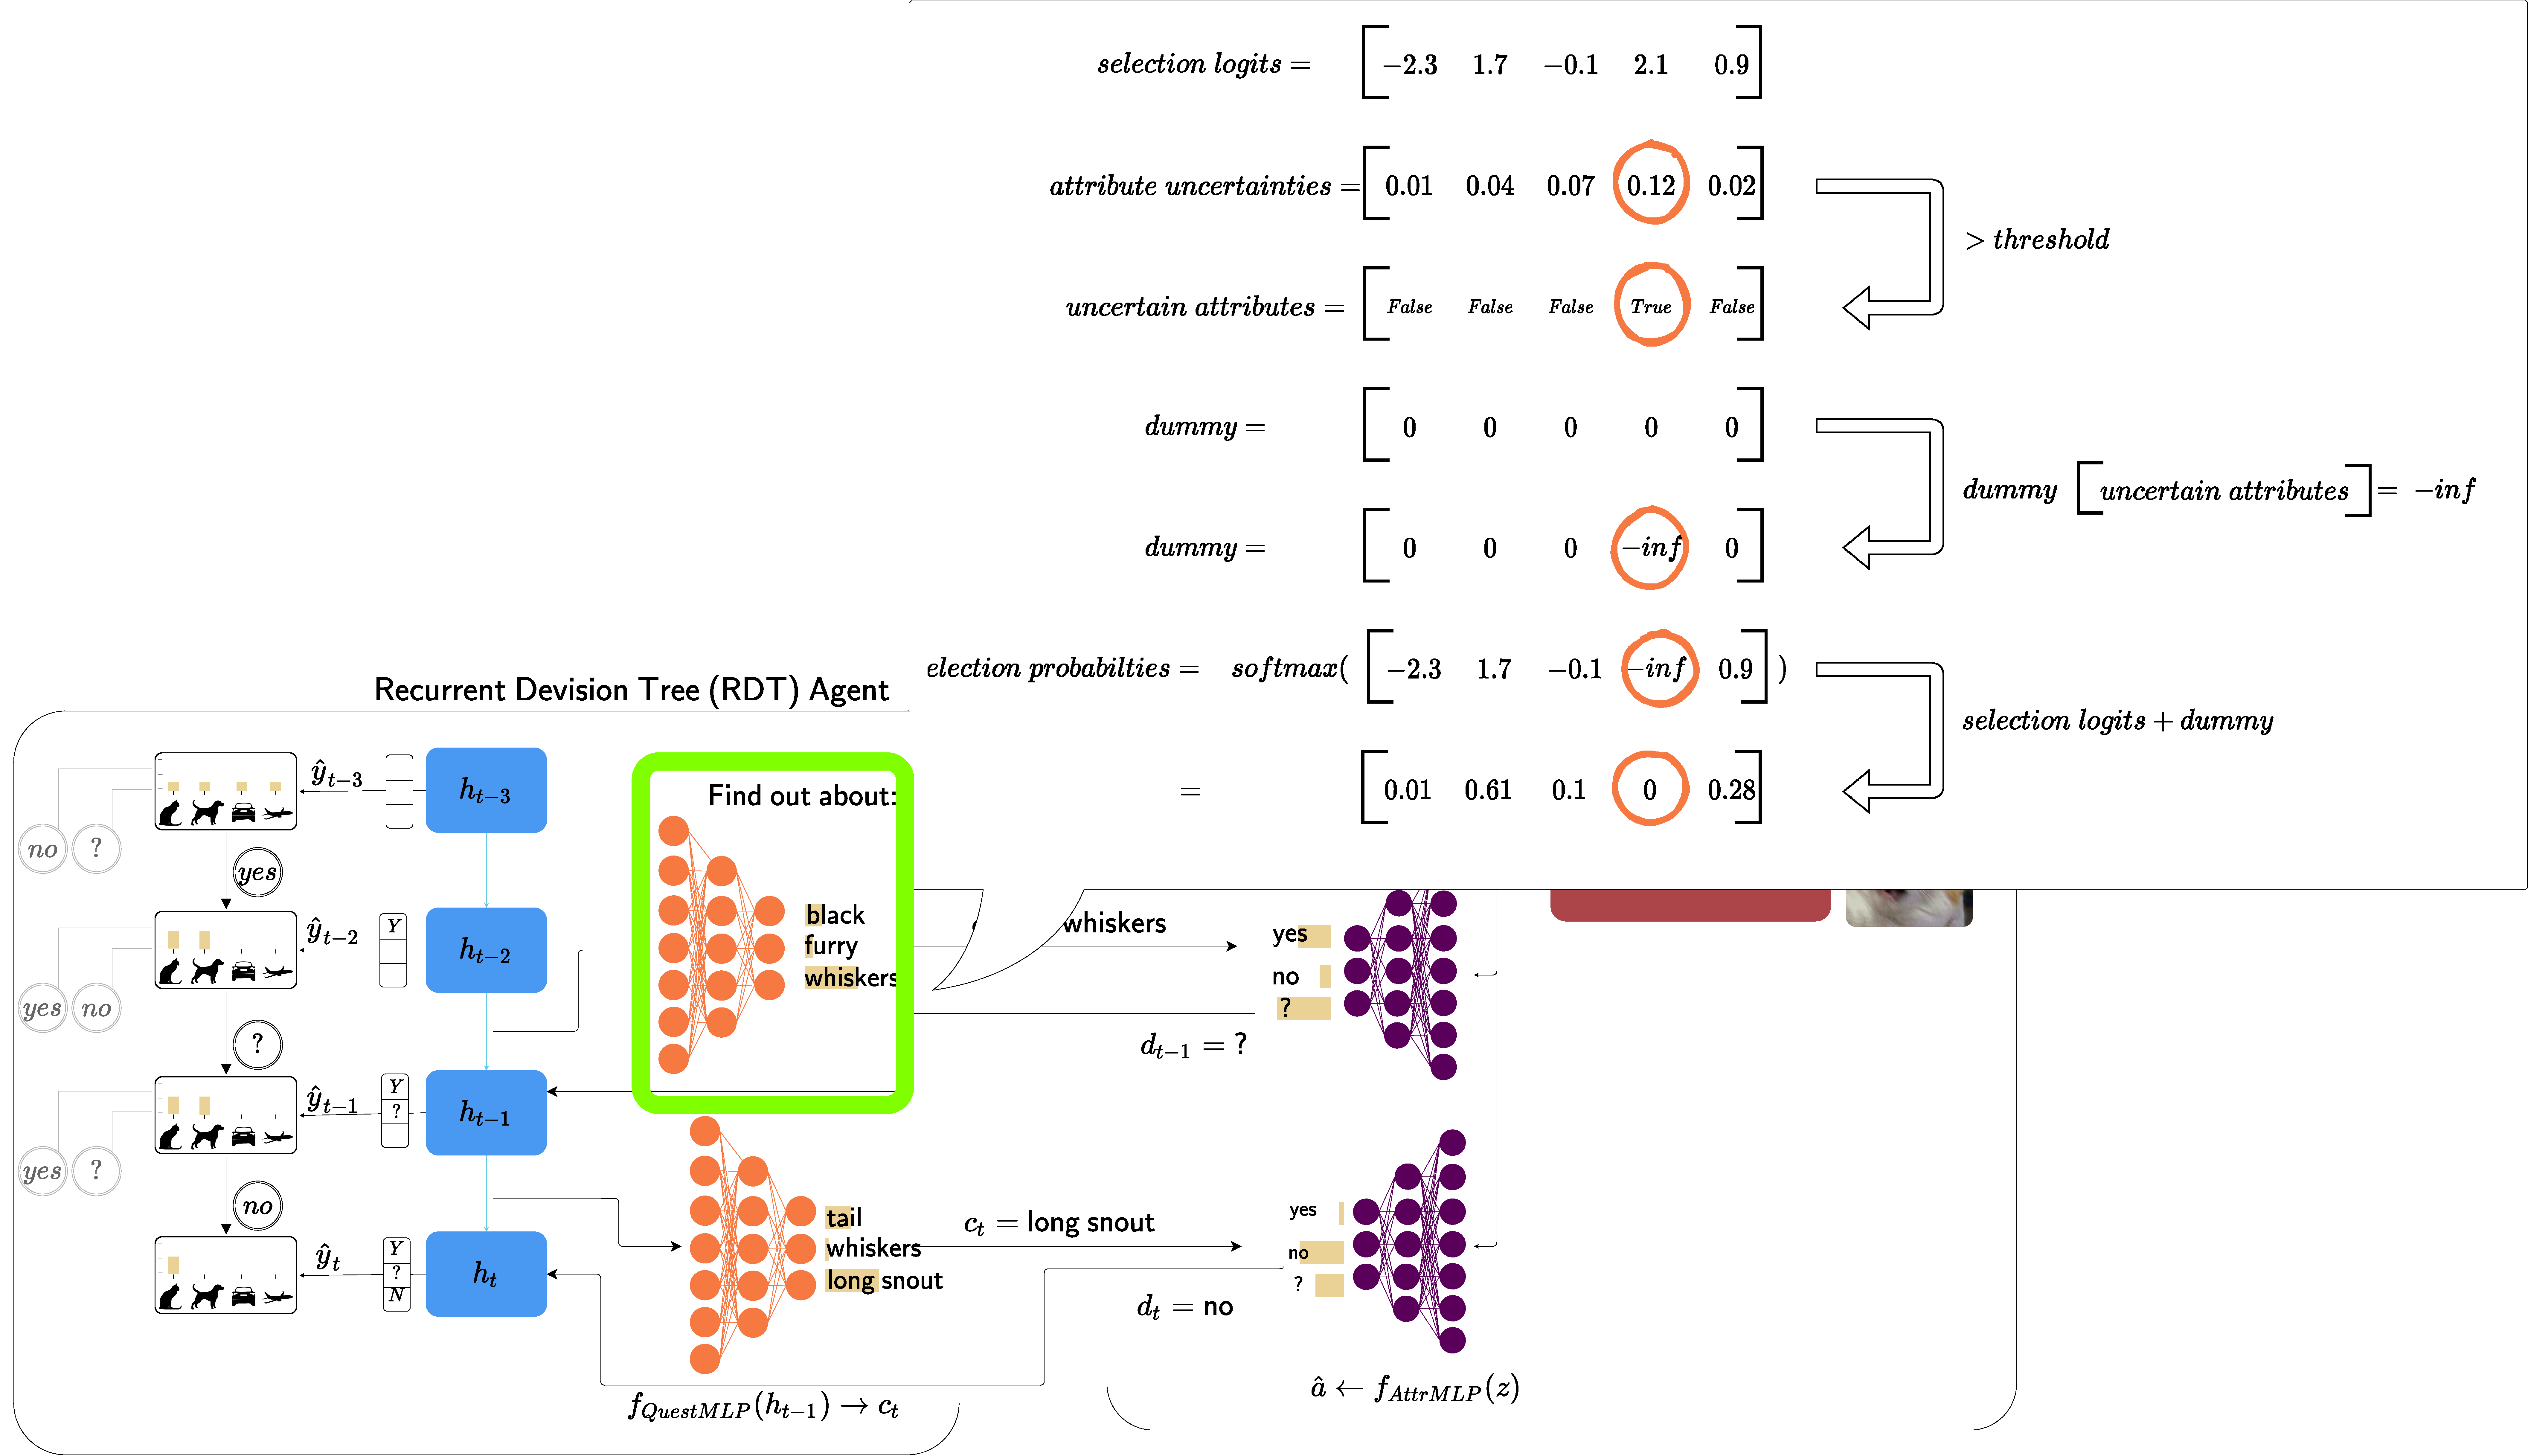
\includegraphics[width=0.8\linewidth]{images/how_to_remRDTC.pdf}
\end{figure}
\begin{itemize}
	\item Reminder: output from $f_{QuestMLP}$ is attribute index %that indicates the attribute in question
	\item If attribute is deemed uncertain by AbL, replace selection logits at those indices with $-\infty$
	\\ $\rightarrow$ Gumbel softmax cannot pick these attributes
\end{itemize}
\end{frame}


\setbeamercolor{background canvas}{bg=white}
\setbeamercolor{normal text}{fg=darkgrey}
\usebeamercolor[fg]{normal text}
\setbeamertemplate{itemize item}{\color{darkgrey}$\circ$}	
\begin{frame}
\frametitle{Using Uncertainty Information}
\framesubtitle{Extending the vocabulary (extRDTC)}
\begin{figure}
	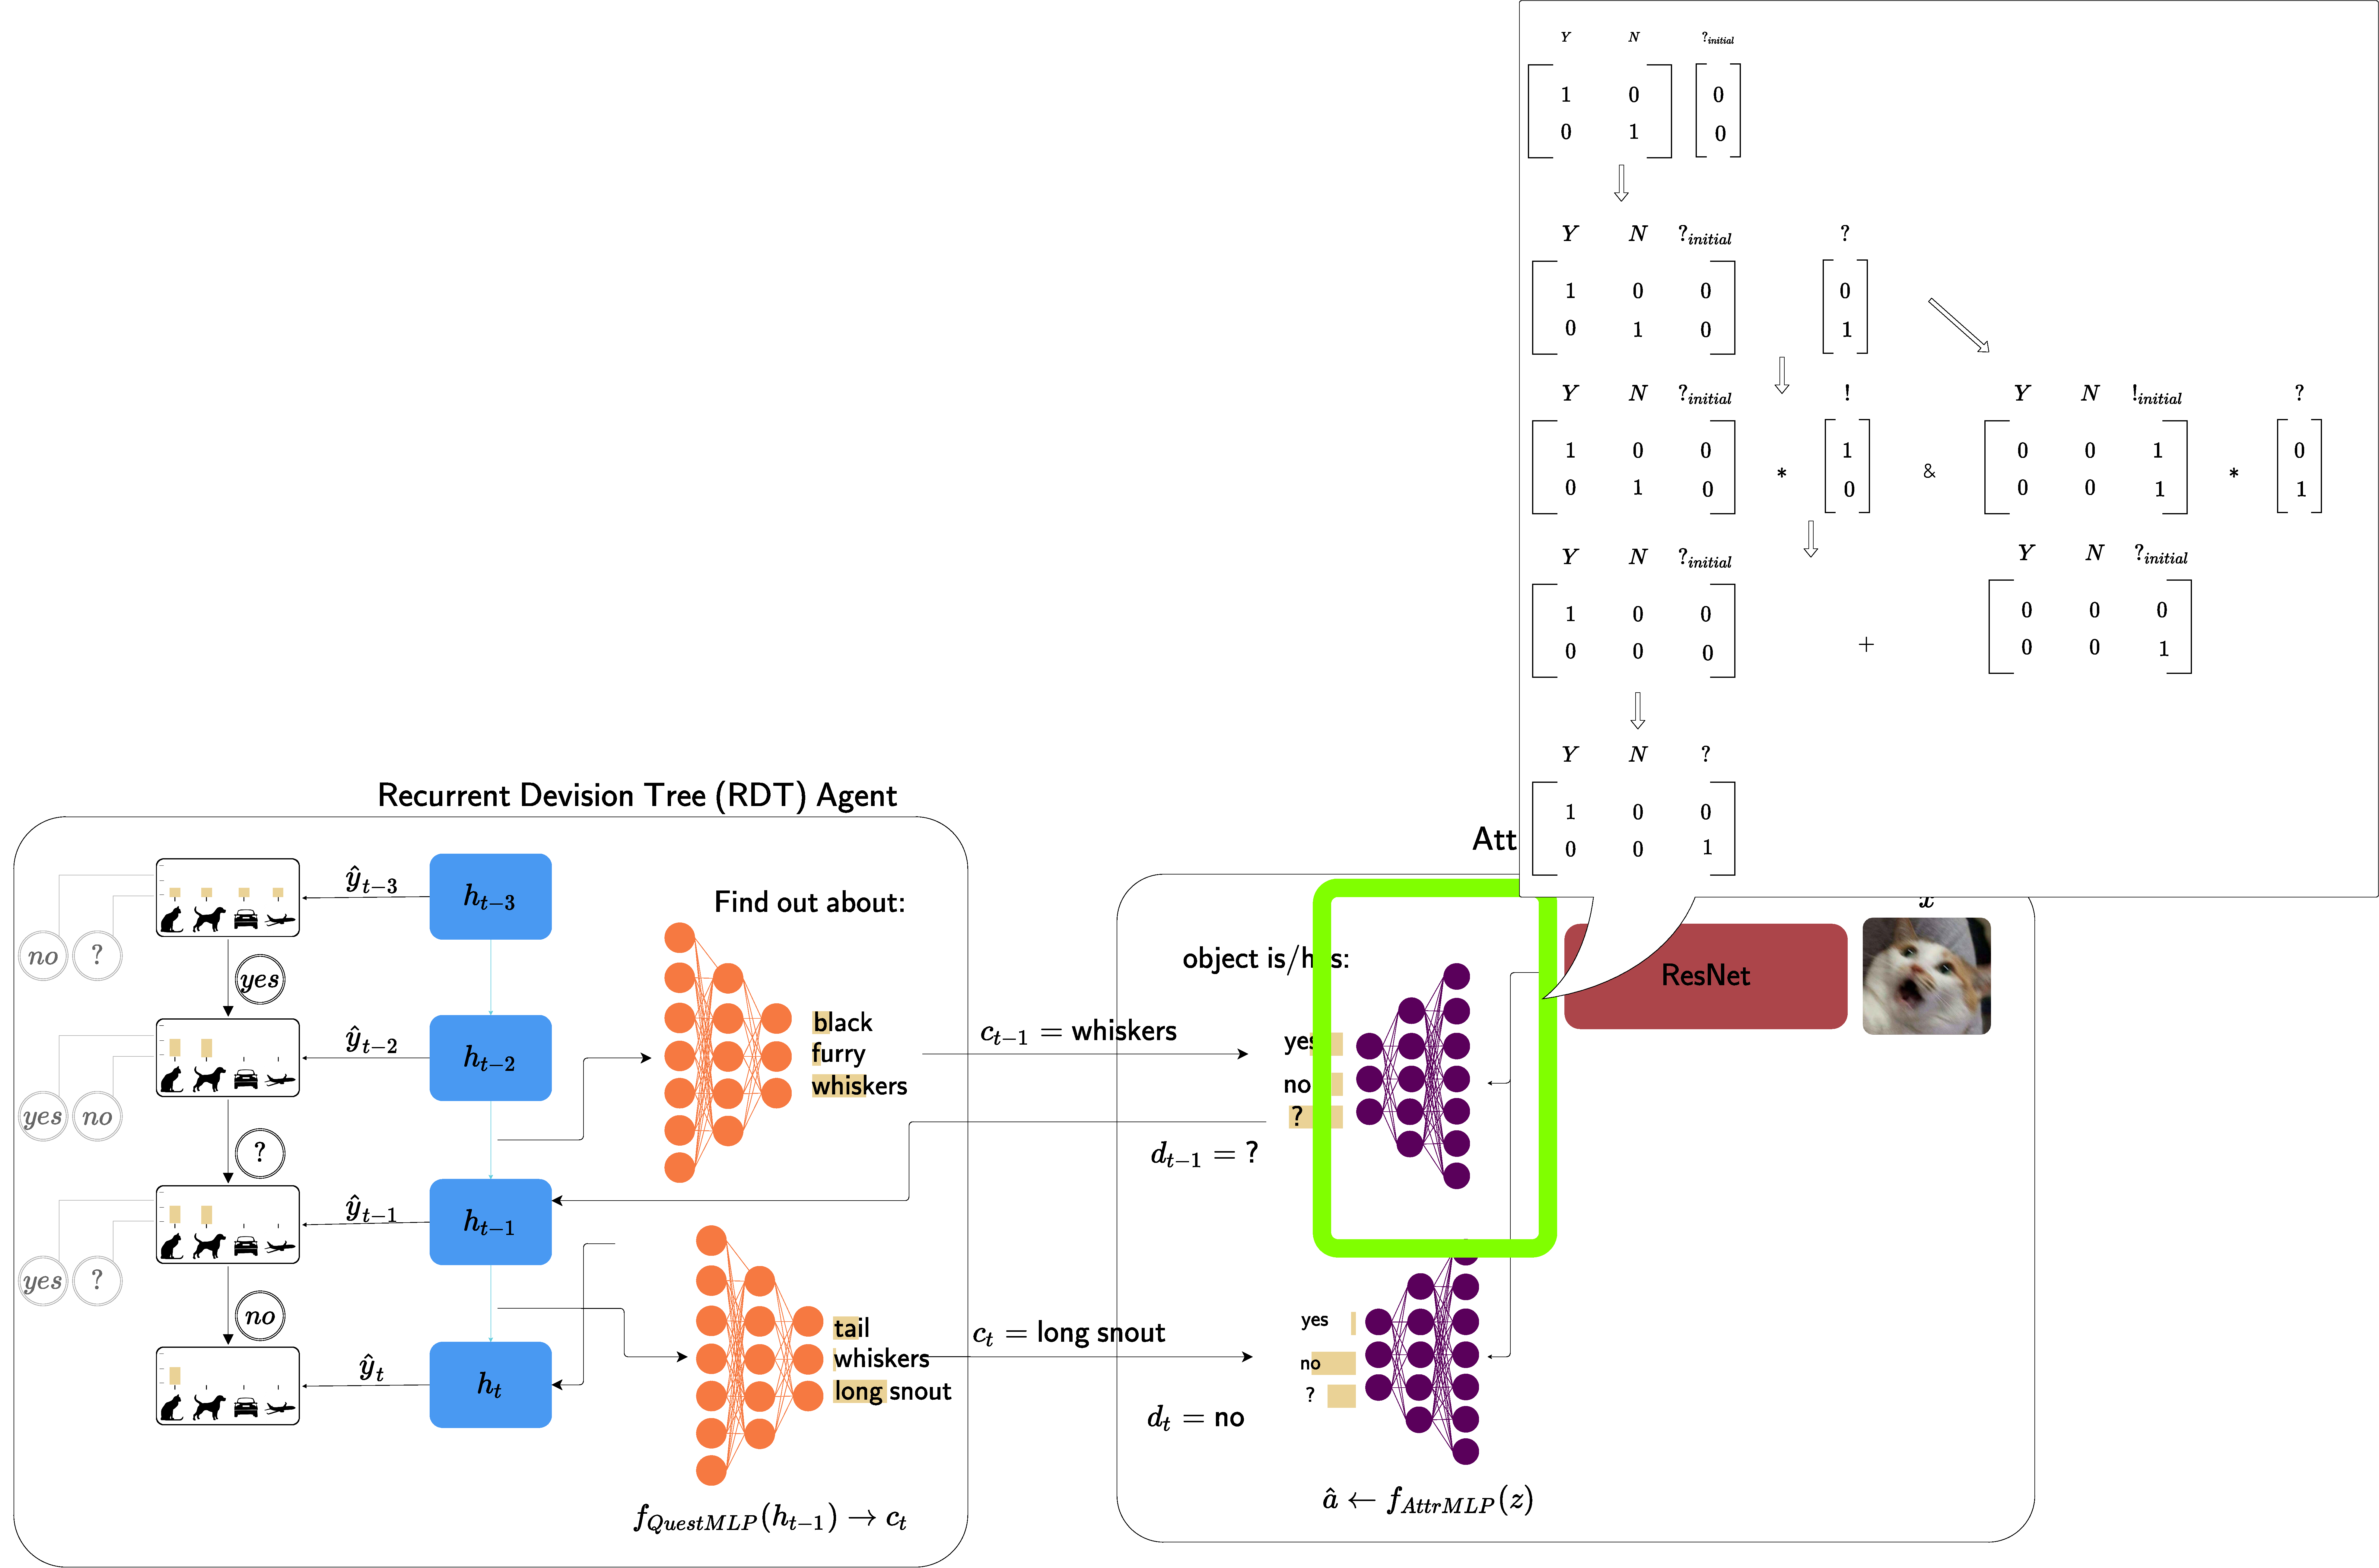
\includegraphics[width=0.8\linewidth]{images/extRDTC_intution.pdf}
\end{figure}
\begin{itemize}
	\item Binary vector with 1s where uncertainty is above threshold
	\item Append to  initial answer% and can be used by the RDT
	\item Prevent conflicting answers
\end{itemize}
\end{frame}



%\setbeamercolor{background canvas}{fg=darkgrey}	
%\setbeamercolor{normal text}{fg=darkgrey}
%\usebeamercolor[fg]{normal text}
%\setbeamertemplate{itemize item}{\color{darkgrey}$\circ$}	
%\begin{frame}
%\frametitle{Using Uncertainty Information}
%\framesubtitle{Extending the vocabulary}
%\begin{figure}
%	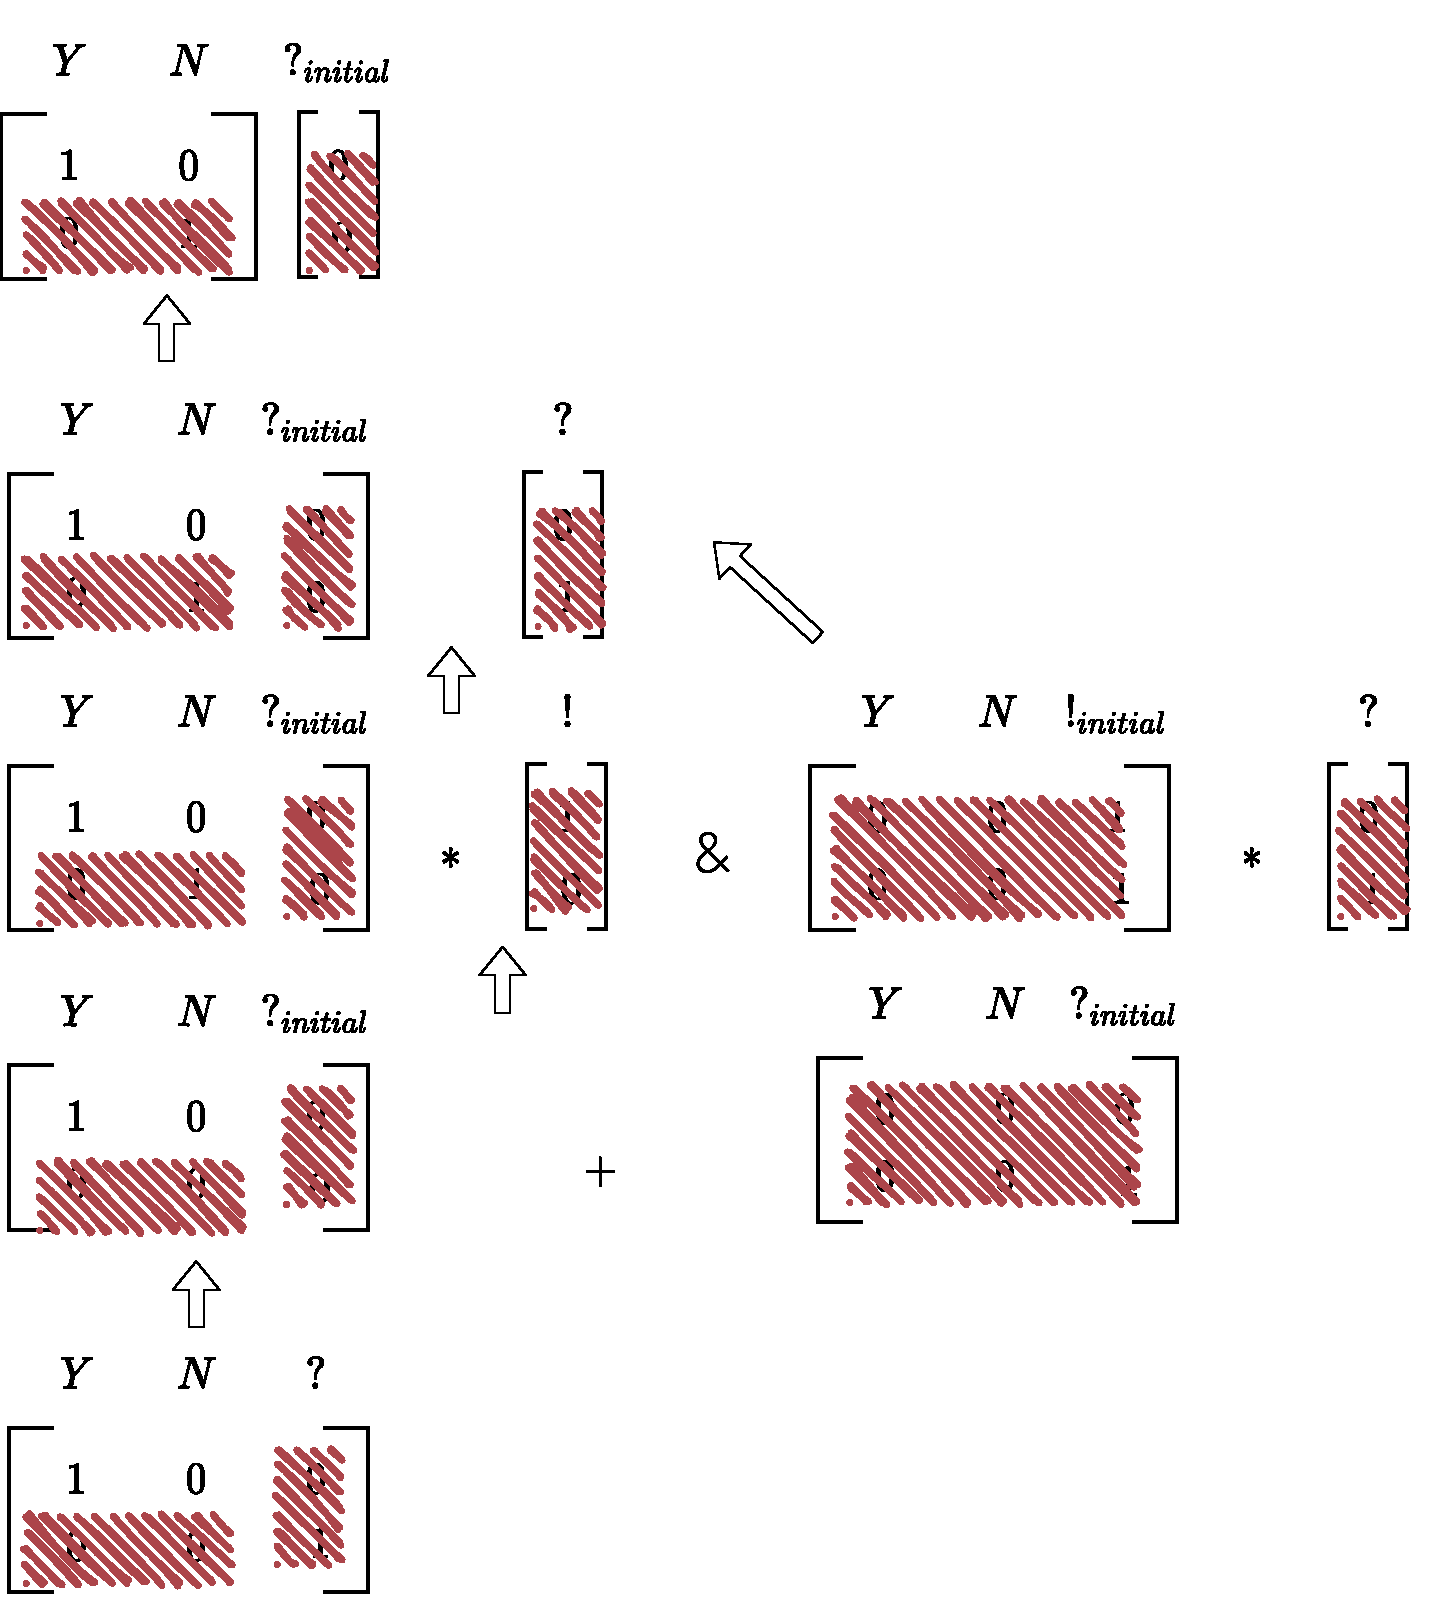
\includegraphics[width=0.6\linewidth]{images/extended_vocab_backward.pdf}
%\end{figure}
%\begin{itemize}
%	\item dsjf
%\end{itemize}
%\end{frame}



\setbeamercolor{background canvas}{bg=orange}
\setbeamercolor{normal text}{fg=white}	
\usebeamercolor[fg]{normal text}
\setbeamertemplate{itemize item}{\color{white}$\circ$}	
\begin{frame}{normal text}
\frametitle{Introducing Uncertainty}
\begin{itemize}
	\item Gal and Ghahramani's \cite{gal2016dropout} proof allows dropout uncertainty estimation
	\item We use their proof to introduce uncertainty to RDTC by Alaniz and Akata \cite{alaniz2019explainable}
	\item Uncertainty information is used in two strategies
	\begin{itemize}
		\item remRDTC
		\item extRDTC
	\end{itemize}
	%\item We use the retrieved uncertainty estimate for either preventing the RDT from asking questions regarding uncertain attributes or extent the AbL's vocabulary
\end{itemize}
\end{frame}





% Experiments
\setbeamercolor{background canvas}{bg=white}
\setbeamercolor{normal text}{fg=darkgrey}
\usebeamercolor[fg]{normal text}
\setbeamertemplate{itemize item}{\color{darkgrey}$\circ$}
\begin{frame}
\frametitle{Experiments}
\framesubtitle{}
\begin{itemize}
	\item RDTC is now aware of, and can express its uncertainties
	\item We use this in our experiments to:
	\begin{itemize}
		\item Investigate uncertainty and its relationship to other variables
		\item Test our model on OOD data
		\item Test the model's performance on benchmark datasets
	\end{itemize}
\end{itemize}
\end{frame}


\setbeamercolor{background canvas}{bg=white}
\setbeamercolor{normal text}{fg=darkgrey}
\usebeamercolor[fg]{normal text}
\setbeamertemplate{itemize item}{\color{darkgrey}$\circ$}	
\begin{frame}
\frametitle{Experiments}
\framesubtitle{Datasets}
\begin{itemize}
	\item Animals with Attributes 2 (AWA2)
	\begin{itemize}
		\item medium size, coarse grained
	\end{itemize}
	\item aPY
	\begin{itemize}
		\item small size, coarse grained
	\end{itemize}	
	\item CUB
	\begin{itemize}
		\item large size, fine grained
	\end{itemize}
\end{itemize}
\end{frame}



\setbeamercolor{background canvas}{bg=white}
\setbeamercolor{normal text}{fg=darkgrey}
\usebeamercolor[fg]{normal text}
\setbeamertemplate{itemize item}{\color{darkgrey}$\circ$}	
\begin{frame}	
\frametitle{Experiments}
\framesubtitle{Investigating Uncertainties in CUB}
\begin{itemize}
	\item Misclassification rate, uncertainty, and usage of attributes
\end{itemize} 
	\begin{figure}
		\centering
		
\includegraphics[width=0.5\textwidth]{images/corr_matrix.pdf}
		%\caption{Correlations between misclassification rate, uncertainty, and usage of attributes.}
		%\label{fig:corr_matrix}
	\end{figure}
	\begin{itemize}
		\item Positive correlation between usage and accuracy
		\item Almost no correlation between uncertainty and accuracy
	\end{itemize}
\end{frame}




\setbeamercolor{background canvas}{bg=white}
\setbeamercolor{normal text}{fg=darkgrey}
\usebeamercolor[fg]{normal text}
\setbeamertemplate{itemize item}{\color{darkgrey}$\circ$}
\begin{frame}	
\frametitle{Experiments}
\framesubtitle{Investigating Uncertainties in CUB}
\begin{itemize}
	%\item Let's have a look at the actual values
	\item Uncertainty, misclassification rate, usage (size $\propto$ usage)
\end{itemize}
	\begin{figure}
		\centering
		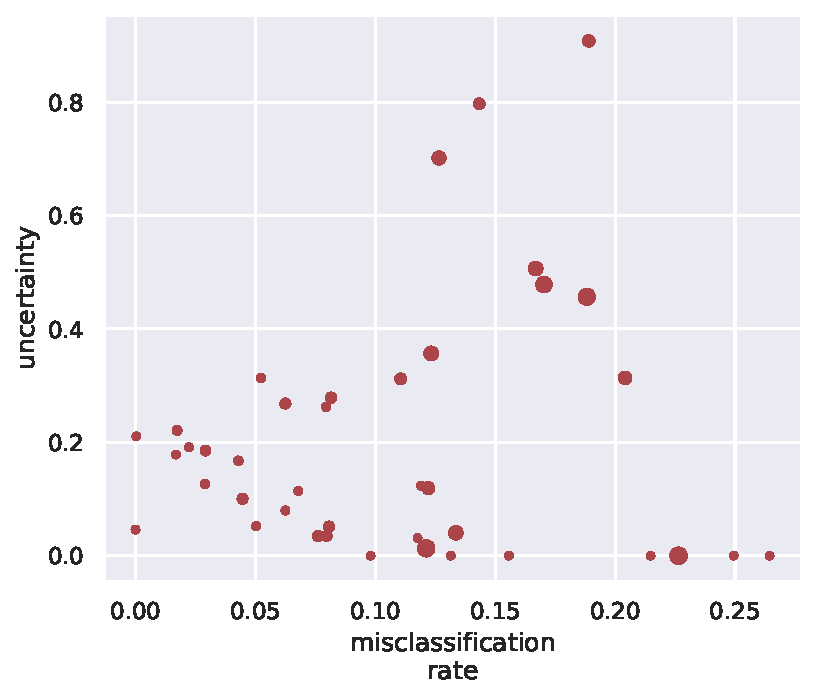
\includegraphics[width=0.5\textwidth]{images/error_sigma_corr_all.pdf} 
		%\caption{Misclassification rates of attributes and their respective uncertainties. The size of the points represents how often they are used.}
		%\label{fig:correlations}
	\end{figure}
	\begin{itemize}
		\item Uncertain attribute seem to be misclassified more often
	\end{itemize}
\end{frame} 



\setbeamercolor{background canvas}{bg=white}
\setbeamercolor{normal text}{fg=darkgrey}	
\usebeamercolor[fg]{normal text}
\setbeamertemplate{itemize item}{\color{darkgrey}$\circ$}	
\begin{frame}
\frametitle{Experiments}
\framesubtitle{OOD Detection}
\begin{itemize}
	\item We test extRDTC in zero shot setting (using CUB)
	\item $\frac{1}{4}$ of classes not seen in training
	\item Histogram of uncertainty values of seen and unseen classes
\end{itemize}
\begin{figure}
	\centering
	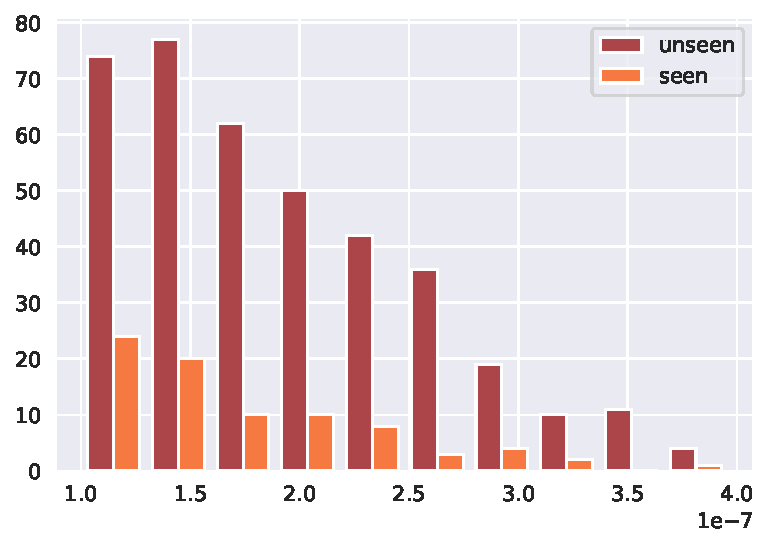
\includegraphics[width=0.5\textwidth]{images/zero_shot_class_uncertainty_median_hist.pdf}
	%\caption{Uncertainty values of attributes from seen and unseen classes. Examples from unseen classes have a higher attribute uncertainty. Attributes with an uncertainty value below $0.0000001$ are not shown.}
\end{figure}
\begin{itemize}
	\item Unseen classes have higher uncertainty values
\end{itemize}
\end{frame} 




\setbeamercolor{background canvas}{bg=white}
\setbeamercolor{normal text}{fg=darkgrey}
\usebeamercolor[fg]{normal text}
\setbeamertemplate{itemize item}{\color{darkgrey}$\circ$}	
\begin{frame}
\frametitle{Experiments}
\framesubtitle{Comparison to other models}
\begin{itemize}
	\item Decision Tree (DT)
	\begin{itemize}
		\item Use extracted ResNet features
		\item Try to split until every leaf node corresponds to one class
	\end{itemize}
	\item Explainable Decision Tree (XDT)
	\begin{itemize}
		\item Same as DT, but using learned attribute representations instead of features
		\item Attribute representations are created using $f_{AttrMLP}$ as head for ResNet
	\end{itemize}	
	\item dNDF \cite{kontschieder2015deep}
	\begin{itemize}
		\item Every node in the tree is a parametric differentiable function
		\item Every route through the tree leads to a leaf node representing a class distribution
		\item Objective is to learn the optimal route through the tree for each example
	\end{itemize}
	\item aRDTC
	\begin{itemize}
		\item RDTC with $\lambda>0$
	\end{itemize}
		\item ResNet
	\begin{itemize}
		\item Not explainable
		\item Trained on ImageNet and then fine-tuned for specific datasets
	\end{itemize}
\end{itemize}
\end{frame}


\setbeamercolor{background canvas}{bg=white}
\setbeamercolor{normal text}{fg=darkgrey}
\usebeamercolor[fg]{normal text}
\setbeamertemplate{itemize item}{\color{darkgrey}$\circ$}	
\begin{frame}
\frametitle{Experiments}
\framesubtitle{Results on Benchmark Datasets}
\begin{table}
	\renewcommand{\arraystretch}{1.3}
	%\caption{We compare accuracy on AWA2, aPY, and CUB of our model and other methods. Standard deviations, denoted by $\pm$ are from five runs.}
	%\label{tab:benchmarks}
	\begin{tabular*}{\textwidth}{c @{\extracolsep{\fill}} c c c c}
		%\hline
		&                                AWA2&          aPY&          CUB\\
		\hline
		\hline
		ResNet \cite{he2016deep}&       98.2$\pm$ 0.0& 85.1$\pm$ 0.6 & 79.0$\pm$ 0.2 \\ 
		\hline 
		DT&                             78.0$\pm$ 0.4&64.3$\pm$ 0.6  & 19.3$\pm$ 0.3  \\ 
		\hline 
		dNDF\cite{kontschieder2015deep}&97.6$\pm$ 0.2&85.0$\pm$ 0.6 & 73.8$\pm$ 0.3 \\ 
		\hline 
		RDTC\cite{alaniz2019explainable}&98.0$\pm$ 0.1&85.7$\pm$ 0.7& 78.1$\pm$ 0.2   \\ 
		\hline 
		XDT&                            73.9$\pm$ 0.9&59.9$\pm$ 1.5  & 4.9$\pm$ 1.3 \\ 
		\hline 
		aRDTC\cite{alaniz2019explainable}&98.6&         86.1&  \textbf{77.9}$\pm$ 0.6\\ 
		\hline
		remRDTC(ours)&          \textbf{98.7}          &          \textbf{86.4}&  77.7\\ 
		\hline
		extRDTC(ours)&          \textbf{98.7}          &          85.4&  77.8\\
		%\hline 
	\end{tabular*}
\end{table}
\end{frame} 



\setbeamercolor{background canvas}{bg=white}
\setbeamercolor{normal text}{fg=darkgrey}
\usebeamercolor[fg]{normal text}
\setbeamertemplate{itemize item}{\color{darkgrey}$\circ$}	
\begin{frame}
\frametitle{Experiments}
\framesubtitle{Results on Benchmark Datasets}
\begin{table}
		\begin{tabular*}{\textwidth}{c  @{\extracolsep{\fill}}c c c c}
		& aRDTC \cite{alaniz2019explainable} & Random Baseline & remRDTC & extRDTC \\ 
		%\hline 
		%\hline
		\textbf{AWA2}& & & &\\\hline\hline
		Class &  \textbf{98.6}&  98.5&  98.7&  98.7\\ 
		\hline 
		Attribute & 80.4 & 84.6 &  \textbf{87.5}&  82.31\\ 
		&  &  &  &  \\
		\textbf{aPY}& & & &\\\hline\hline
		Class & 86.1&  \textbf{86.5}&  86.4&  85.4\\ 
		\hline 
		Attribute &  86.4&  86.2&  \textbf{87.6}& 87.1 \\ 
		&  &  &  &  \\ 
		\textbf{CUB}& & & &\\\hline\hline
		Class &  \textbf{77.9}& 76.8 & 77.7 & 77.8 \\ 
		\hline
		Attribute &  68.6&  70.0& 77.4 & \textbf{82.6} \\ 
		&  &  &  &  \\ 
	\end{tabular*}
\end{table}
\end{frame} 



\setbeamercolor{background canvas}{bg=orange}
\setbeamercolor{normal text}{fg=white}
\usebeamercolor[fg]{normal text}
\setbeamertemplate{itemize item}{\color{white}$\circ$}
\begin{frame}
\frametitle{Experiments}
\begin{itemize}
	\item RDTC prefers attributes that it rarely misclassifies
	\item Uncertain attributes seem to be misclassified more often
	\item Unseen classes yield higher uncertainty
	\item Both remRDTC and extRDTC perform well on benchmark tasks
\end{itemize}
\end{frame}
%\setbeamertemplate{background canvas}{bg=white}

\setbeamercolor{background canvas}{bg=white}
\setbeamercolor{normal text}{fg=darkgrey}
\usebeamercolor[fg]{normal text}
\setbeamertemplate{itemize item}{\color{darkgrey}$\circ$}	
\begin{frame}
\frametitle{Discussion}
\framesubtitle{Looking back...}
\begin{itemize}
	\item The right kind of uncertainty?
	\begin{itemize}
		%\item We only consider model uncertainty (epistemic uncertainty)
		\item Uncertainty arising from noise or occlusions is not considered
		\item Dropout Uncertainty Estimation lacks empirical proof
	\end{itemize}
	\item Other methods of uncertainty estimation%/ Approximated BNN's
	\begin{itemize}
		\item Often computationally expensive
		\item Open area of research
	\end{itemize}
	\item Beyond attribute uncertainty
	\begin{itemize}
		\item Estimate uncertainty in other parts of the model (i.e. $f_{ClassMLP}$)
	\end{itemize}
\end{itemize}
\end{frame} 










% Conclusion
\setbeamercolor{background canvas}{bg=white}
\setbeamercolor{normal text}{fg=darkgrey}
\usebeamercolor[fg]{normal text}
\setbeamertemplate{itemize item}{\color{darkgrey}$\circ$}
\begin{frame}
\frametitle{Conclusions}
\framesubtitle{A qualitative Example}
\begin{figure}
	\centering
	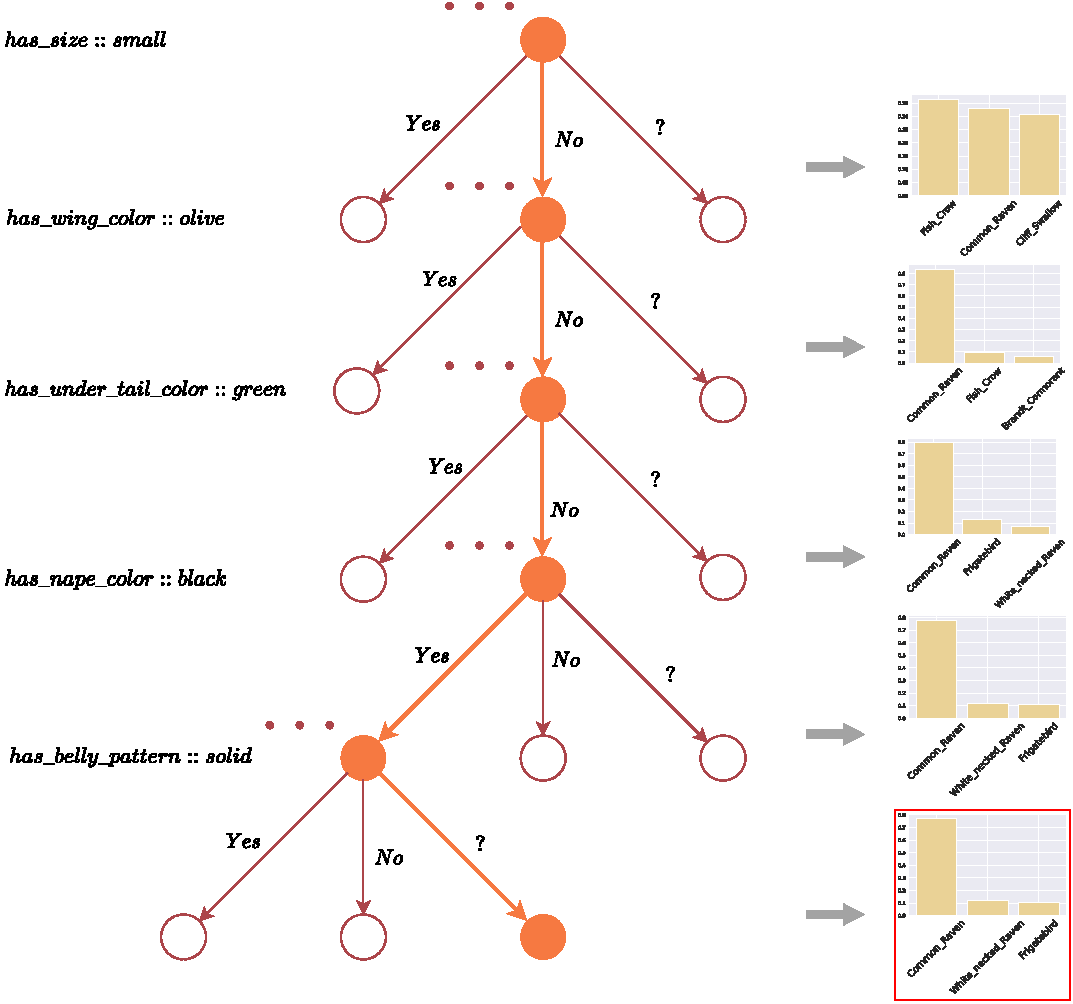
\includegraphics[width=0.7\textwidth]{images/example_tree.pdf}
%\caption{Five steps of a extRDTC decision process. The model has used an uncertain attribute and the final classification is wrong. In such a case, a human user could be consulted and manually classify the image. Note that the the softmax classification output is highly confident despite being wrong.}
\label{fig:example_tree}
\end{figure}
\end{frame} 







\setbeamercolor{background canvas}{bg=orange}
\setbeamercolor{normal text}{fg=white}
\usebeamercolor[fg]{normal text}
\setbeamertemplate{itemize item}{\color{white}$\circ$}
\begin{frame}
\frametitle{Conclusions}
%\framesubtitle{}
\begin{itemize}
	\item Based on proof by Gal and Ghahramani \cite{gal2016dropout} estimate uncertainty
	\item Uncertainty is used in RDTC by Alaniz and Akata \cite{alaniz2019explainable}
	\item Two strategies: remRDTC and extRDTC
	\item We investigate uncertainty and its relationship to other variables
	\item We show that OOD examples yield high uncertainty
	\item Uncertain RDTC's achieve state of the art accuracy
\end{itemize}
\end{frame}




\setbeamercolor{background canvas}{bg=white}
\setbeamercolor{normal text}{fg=darkgrey}
\usebeamercolor[fg]{normal text}
\setbeamertemplate{itemize item}{\color{darkgrey}$\circ$}
\begin{frame}
\frametitle{References}
	\bibliographystyle{alpha}
	\bibliography{bibliography}
\end{frame}


\end{document}
